\chapter{Experiment}
\label{chp:exp}

This chapter provides an overview of the experimental setup of the LHC collider and the CMS detector. A brief description of the LHC is given in the Section~\ref{sec:exp:lhc}, followed by introductions to the CMS detector apparatus, triggering system and object reconstruction in the Section~\ref{sec:exp:apparatus}, \ref{sec:exp:trigger} and \ref{sec:exp:reco}, respectively, mainly based on a collection of CMS technical design reports (TDRs) \cite{cms:tdr1:Bayatian:2006nff , cms:tdr2:Ball:2007zza , cms:magnetTdr:Acquistapace:1997fm , cms:trackerTdr:CMS:1997tlf , cms:ecalTdr:CMS:1997ysd , cms:hcalTdrCMS:1997xji , cms:muonChamberTdr:CMS:1997iti} and CMS papers about the experiment \cite{exhep:cms:Chatrchyan:2008aa}, triggering system \cite{cms:trigger:Khachatryan:2016bia}, particle-flow algorithms \cite{cms:particleflow:Sirunyan:2017ulk}.




% ---------------------------------------
% section : Large Hadron Collider
% ---------------------------------------
\section{Large Hadron Collider}
\label{sec:exp:lhc}

% overview
The \acrfull{lhc} \cite{exhep:lhc:Evans:2008zzb} is a 27 \si{\km} circular particle collider located at the \acrfull{cern} across the border between France and Switzerland. The LHC was constructed during 1998-2008 in a 100-meter-deep underground tunnel previously used by the \acrfull{lep} \cite{exhep:lep:Myers:1991ym}. Inside the LHC, two proton beams collide at a maximum center-of-mass energy of $\sqrt{s}=14$ TeV with a designed instant luminosity of \SI{e34}{\per\cm\squared \per\s}. Around the ring path of the LHC, four collision positions are designed corresponding to four LHC experiments: CMS \cite{exhep:cms:Chatrchyan:2008aa} (Point 5), ATLAS \cite{exhep:atlas:Aad:2008zzm} (Point 1), LHCb \cite{exhep:lhcb:Alves:2008zz} (Point 8) and Alice \cite{exhep:alice:Aamodt:2008zz} (Point 2).


% constituents
The main components of LHC include two tubes with ultrahigh vacuum and about ten thousand superconducting magnets with various sizes installed alone the ring, including 1232 dipole magnets with length of 15 \si{\m} to bend the beams and 392 quadrupole magnets with length of 5-7 \si{\m} to focus the beams \cite{exhep:lhcFactsFigures}. Magnets of higher multipole orders are also used for corrections of the magnetic field. A liquid helium cooling system is used to cool the superconducting electromagnets at a cryogenic temperature of -271.3 \si{\degreeCelsius}. 


\begin{figure}[ht]
    \centering
    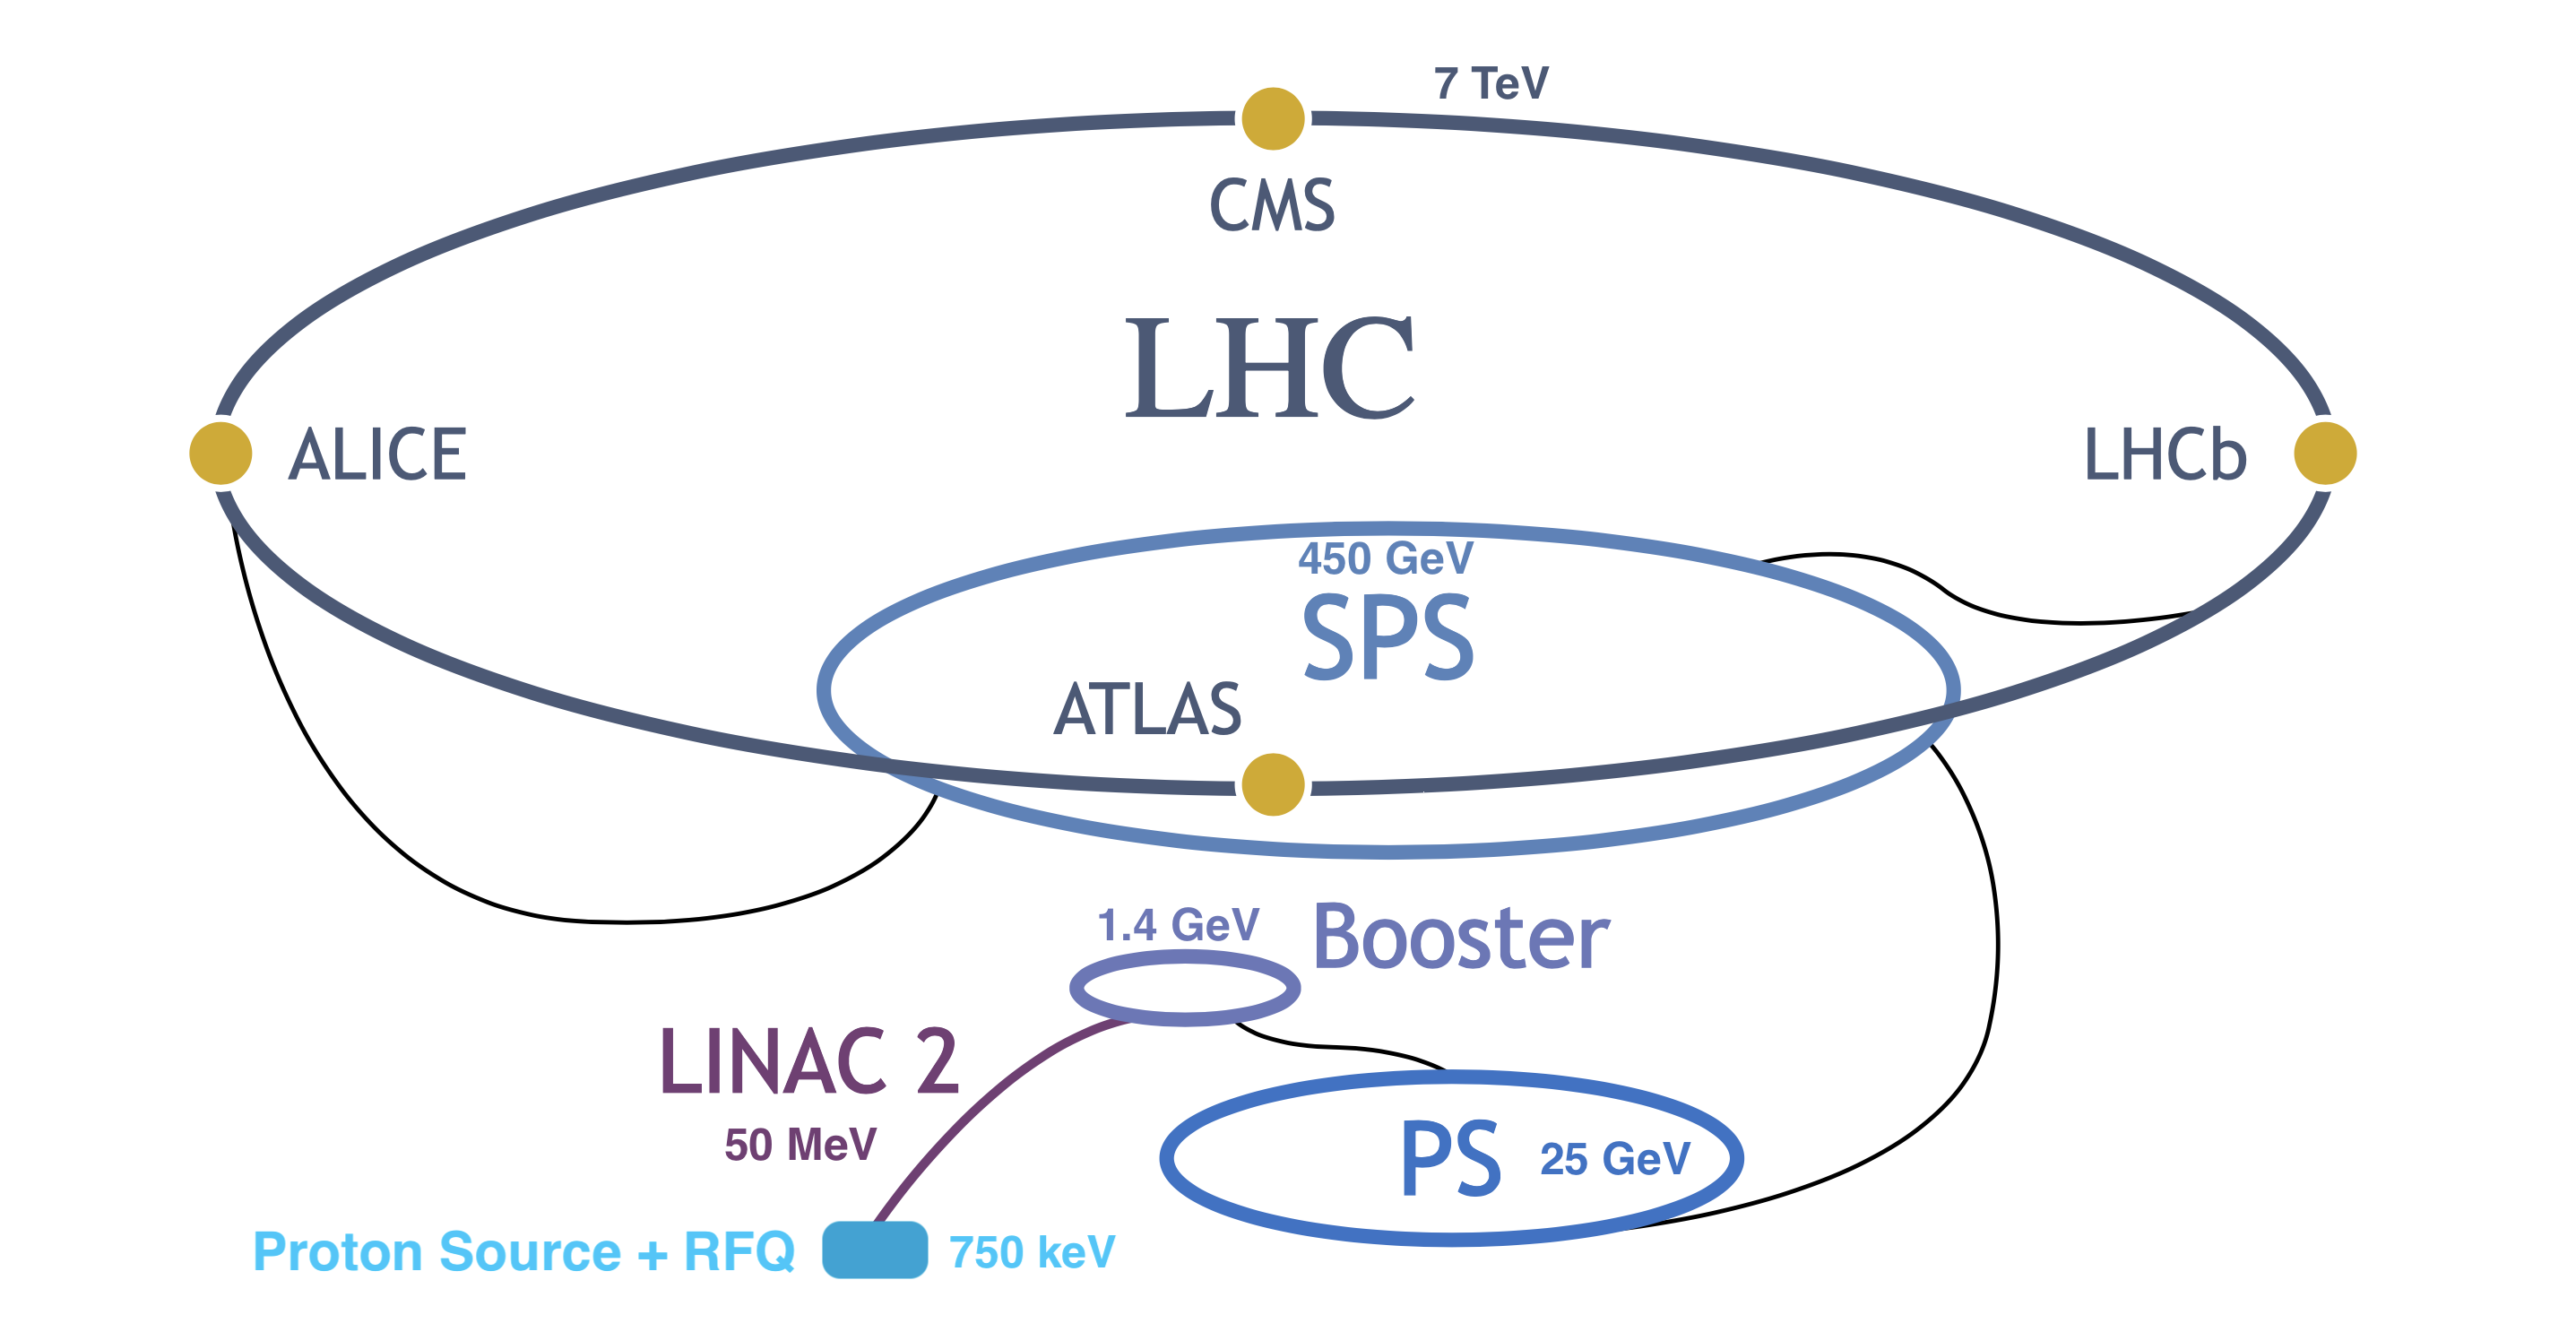
\includegraphics[width=0.8\textwidth]{chapters/2_experiment/figures/lhc.png}
    \caption{Schematic overview of the LHC and related accelerator complex: chain of proton source, RFQ, LINAC2, PSB, PS, SPS, LHC \cite{exhep:lhcInject:Benedikt:2004wm}.}
    \label{fig:exp:lhc}
\end{figure}


% beam pipe
Before injected into the LHC, protons are accelerated to 450 GeV by a few existing accelerator facilities at CERN. Figure~\ref{fig:exp:lhc} shows a schematic overview of the LHC with its related accelerator complex at CERN \cite{exhep:lhcInject:Benedikt:2004wm}. First, protons are produced by the ionization hydrogen gas and are extracted by a 90 keV voltage to inject into the \acrfull{rfq} where protons are divided into bunch crossings and are accelerated to 750 keV. A linear accelerator (Linac2) then energizes them to 50 MeV. The \acrfull{psb}, which has four superimposed synchrotron rings, brings the protons to 1.4 GeV for the injection to the \acrfull{ps}, a 628 \si{\m} synchrotron outputing beams with energy of 25 GeV. The \acrfull{sps} further boosted to 450 GeV in its 7-\si{km}-long ring and deliver the beam to LHC. When accelerating proton beam from 450 GeV at the LHC injection to 6.5 TeV for the physics collision in the Run-2, the dipole magnetic field is increased from 0.54 \si{\tesla} to 7.7 \si{\tesla} to increase the banding power to circulating energized beams. During a physics run, luminosity of LHC decays with a lifetime about 14.9 hours \cite{exhep:lhc:Evans:2008zzb} due to effects of physics cross-section, photon emittances alone the circular path and scattering off the air remains. Therefore, every one or two days



% operation schedule
The operation of LHC from 2010 to 2035 consists of 6 runs with shutdown periods for upgrading and maintenance during the run intervals. In the Run-1 from 2010 to 2013, LHC delivered about 6 $fb^{-1}$ pp collision at $\sqrt{s}=7$ TeV in 2010, 2011 and 23.3 $fb^{-1}$ pp collision at $\sqrt{s}=8$ TeV in 2012 \cite{cms:publicLumiInfo}, with which the discovery of Higgs boson was made by the ATLAS \cite{exhep:atlasHiggsDisc:Aad:2012tfa} and the CMS \cite{exhep:cmsHiggsDisc:Chatrchyan:2012ufa}. In the Run-2 from 2016 to 2018, LHC produced 144 $fb^{-1}$ pp collisions at $\sqrt{s}=13$ TeV \cite{cms:publicLumiInfo}. Currently in 2020, the LHC is in its second long shutdown period, expecting Run3 starting in 2021 to operate at the maximum collision energy of $\sqrt{s}=14$ TeV. After Run3, LHC will be upgraded to higher luminosity or the \acrfull{hllhc} to reach an instant luminosity of \SI{5e34}{\per\cm\squared \per\s}, five times as much as current value. In the era of HL-LHC, three extra runs are scheduled during 2026-2035. In the long term future beyond the HL-LHC era, the \acrfull{fcc} \cite{exhep:fcc:Benedikt:2715354} plan is proposed to build a 100 km hadron collider next to the LHC and further increase the collision energy to the level of 100 TeV.



% ---------------------------------------
% section : Detector Apparatus
% ---------------------------------------

\section{Detector Apparatus}
\label{sec:exp:apparatus}

% overview
The CMS \cite{exhep:cms:Chatrchyan:2008aa} detector is a general-purpose apparatus operating at the LHC and is located about 100 meters underground at Point 5 of the LHC, close to the French village of Cessy, between Lake Geneva and the Jura mountains. As a general purpose detector, the CMS detector is designed to observe any new physics phenomena that the LHC might reveal \cite{cms:tdr2:Ball:2007zza}. At the designed LHC luminosity of \SI{e34}{\per\cm\squared \per\s}, on average about 20 inelastic collisions are superimposed on the event of interest every collision of bunch crossings, leading to a large flux of particles originating from the detector center to enter the detector every 25 ns. In order to discern them and trigger the interested events within 25 ns latency over the LHC run period until 2035, CMS detector is designed to be highly-segmented, radiation-hard and with good timing resolution \cite{exhep:cms:Chatrchyan:2008aa}.

\begin{figure}[ht]
    \centering
    \includegraphics[width=0.98\textwidth]{chapters/2_experiment/figures/cmsDetector.png}
    \caption{The layout of the CMS detector \cite{cms:detectorOverview}.}
    \label{fig:exp:detectorOverview}
\end{figure}

% overview of structure
The apparatus layout of CMS detector is shown in Figure~\ref{fig:exp:detectorOverview} \cite{cms:detectorOverview}. The central feature of the CMS apparatus is a superconducting solenoid of 6 m internal diameter, providing a magnetic field of 3.8 T. Within the superconducting solenoid volume are a silicon pixel and strip tracker, a lead tungstate crystal electromagnetic calorimeter, and a brass and scintillator hadron calorimeter, each composed of a barrel and two endcap sections. Muons are measured in gas-ionization detectors embedded in the steel flux-return yoke outside the solenoid. Additional forward calorimetry complements the coverage provided by the barrel and endcap detectors. The more details of these sub-systems, including magnet,  are discussed in this section. 

% To achieve the physics goal in the LHC environment, the design of each CMS sub-detectors are driven by the following performance requirement.

% \begin{itemize}
%     \item Magnets and Muon chamber: Good muon identification, energy resolution, charge determination.
%     \item Pixel and Tracker: Good charge hadron track reconstruction efficiency. Good displaced vertex tagging for $b$, $\tau$ identification.
%     \item ECAL: Good electromagnetic energy resolution. $\pi^0$ rejection. Efficient photon and lepton isolation at high luminosities.
%     \item HCAL: Good missing-transverse-energy and dijet-mass resolution
% \end{itemize}



\subsection{Magnet}
% overview
The CMS superconducting magnet \cite{cms:magnetTdr:Acquistapace:1997fm} is used to provide bending to the charged particles as they traverse, which is crucial to both particle identification and momentum measurement. The internal magnetic filed is 4 Tesla with 2.6 GJ stored energy and is generated by a superconducting solenoid surrounded by a set of return york. The solenoid is 12.5 m in length, 6.3 m in diameter and 200 ton in weight, consist of 41.7 MA-turn of wire. The radiation thickness of the solenoid is 4.9 $\chi_0$, which further prevents hadrons from entering the muon system. The solenoid is surrounded and mechanically supported by the iron return yokes, which direct the outer magnetic in the muon system. The yoke, consist of 5 barrel wheels and two endcaps, has an outer diameter of 14 m and a total weight of 10000 tons. Both barrel and endcap return yoke have three iron layers with thickness of 300/630/630 mm and 250/600/600 mm, respectively.



\subsection{Inner Tracking System}
% overview
The inner tracking system \cite{cms:trackerTdr:CMS:1997tlf} is used to measure the trajectories of charged particles. Covering region with $|\eta|<2.5$, it is consist of two major parts: pixel detector and Silicon strip tracker, layout of which is shown in Figure~\ref{fig:exp:trigger}. 


\begin{figure}[ht]
    \centering
    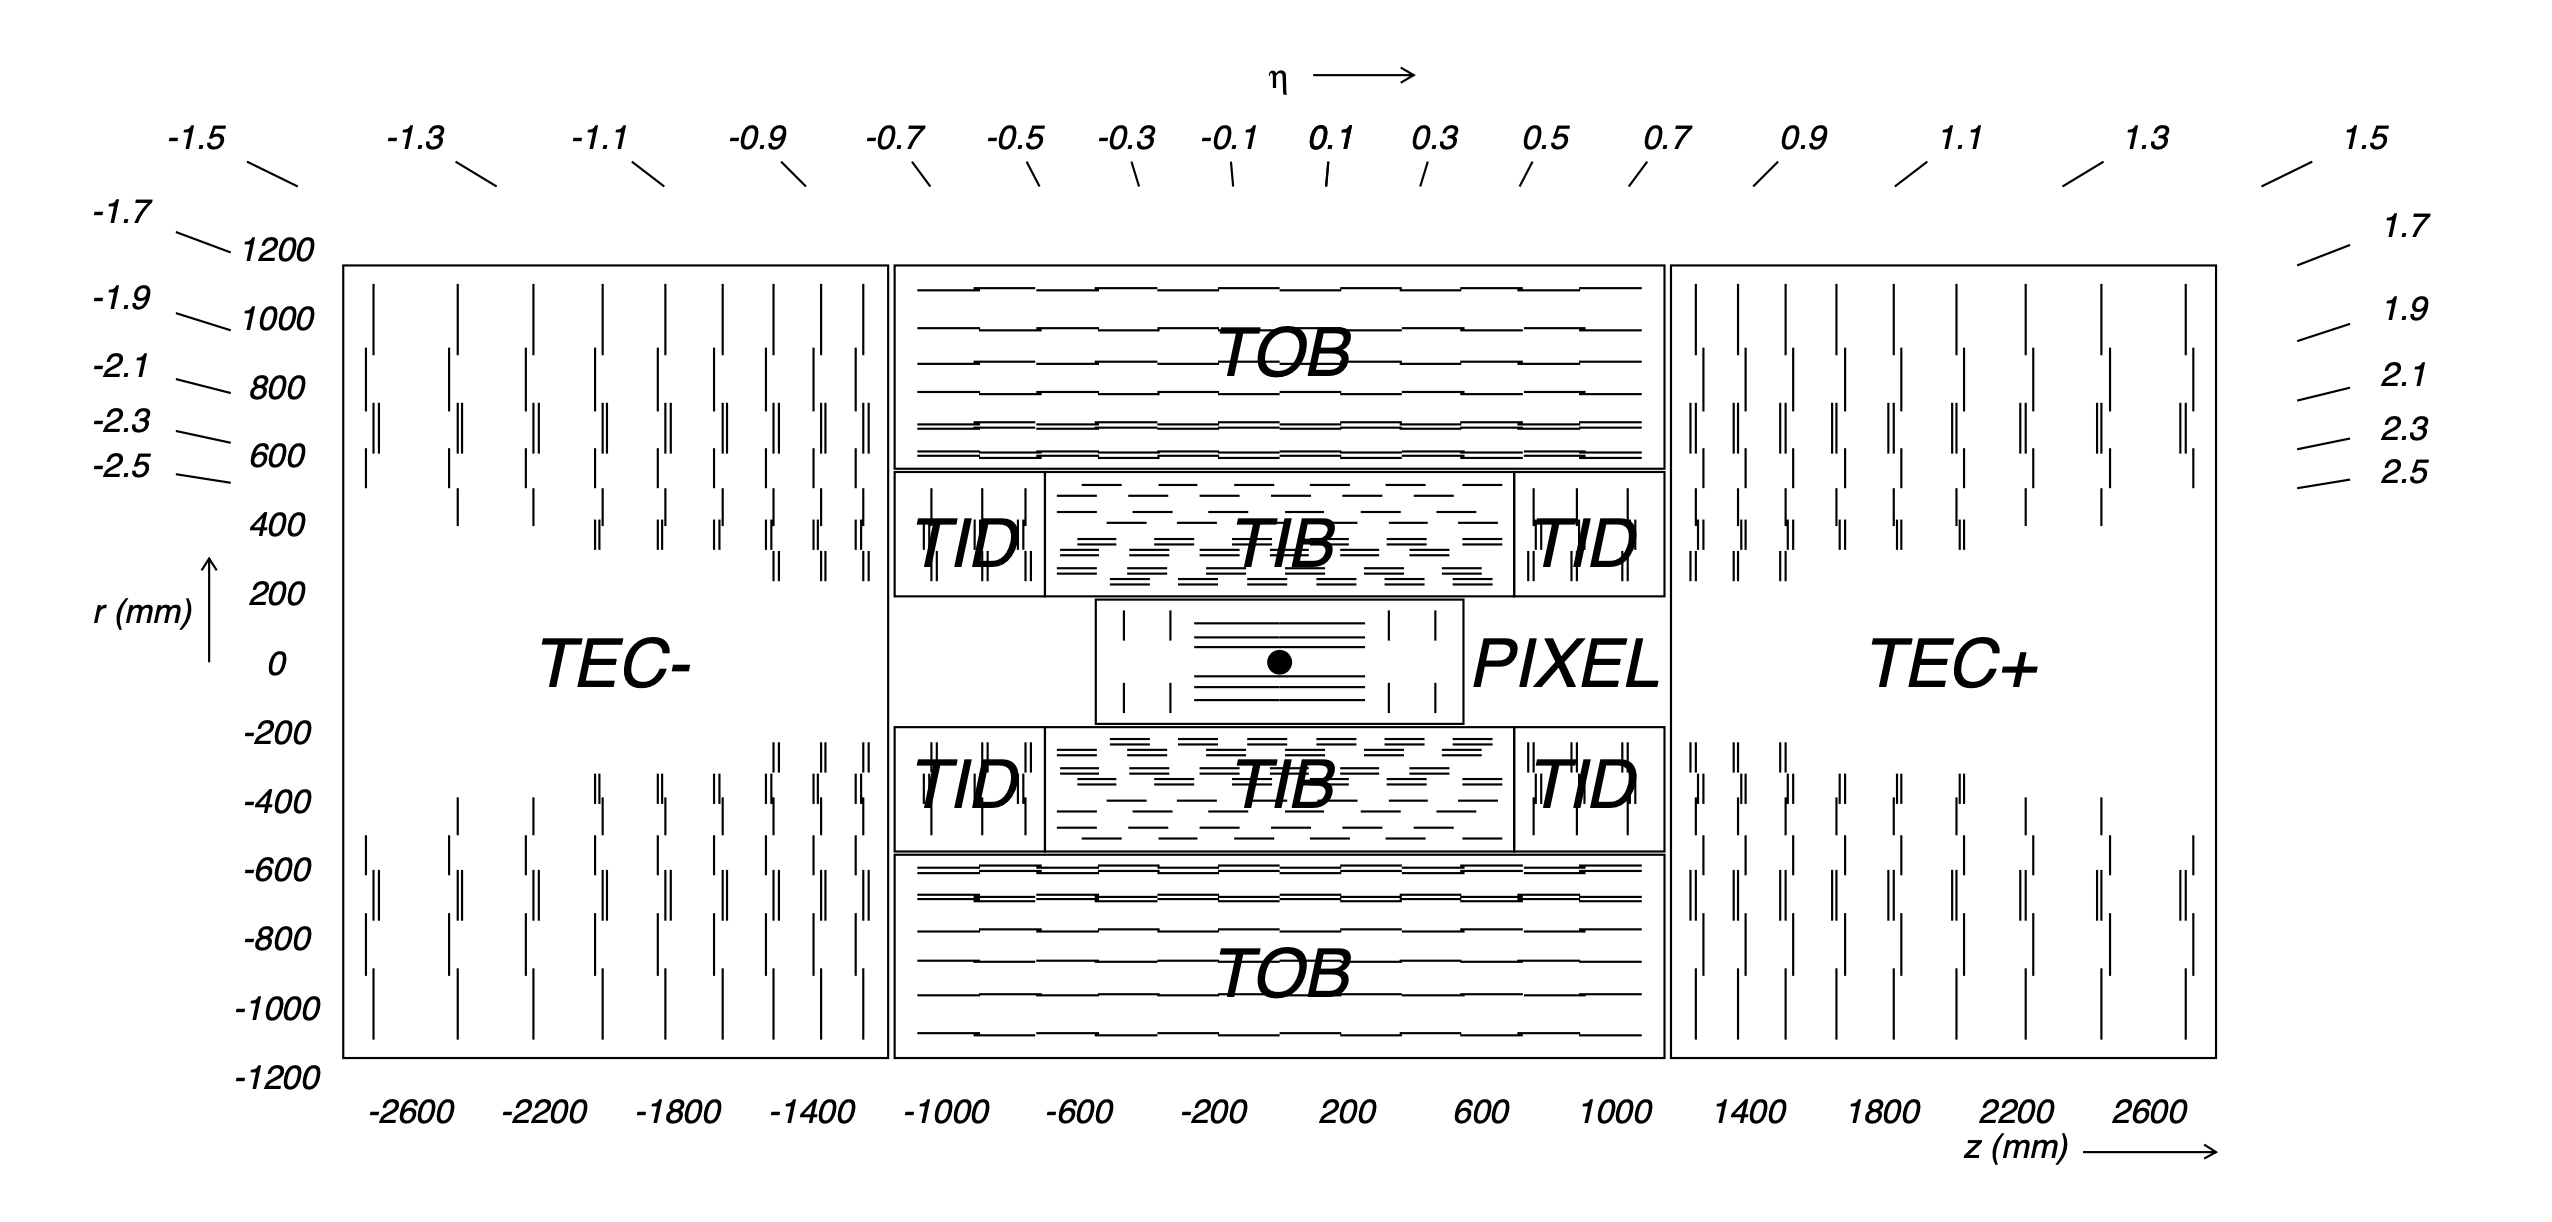
\includegraphics[width=0.98\textwidth]{chapters/2_experiment/figures/tracker.png}
    \caption{The layout of the CMS inner tracking system \cite{exhep:cms:Chatrchyan:2008aa}. It is consist of pixel detector and silicon strip tracker (TIB/TID, TOB, TEC), covering regions with $|\eta|<2.5$. }
    \label{fig:exp:tracker}
\end{figure}


\begin{figure}[ht]
    \centering
    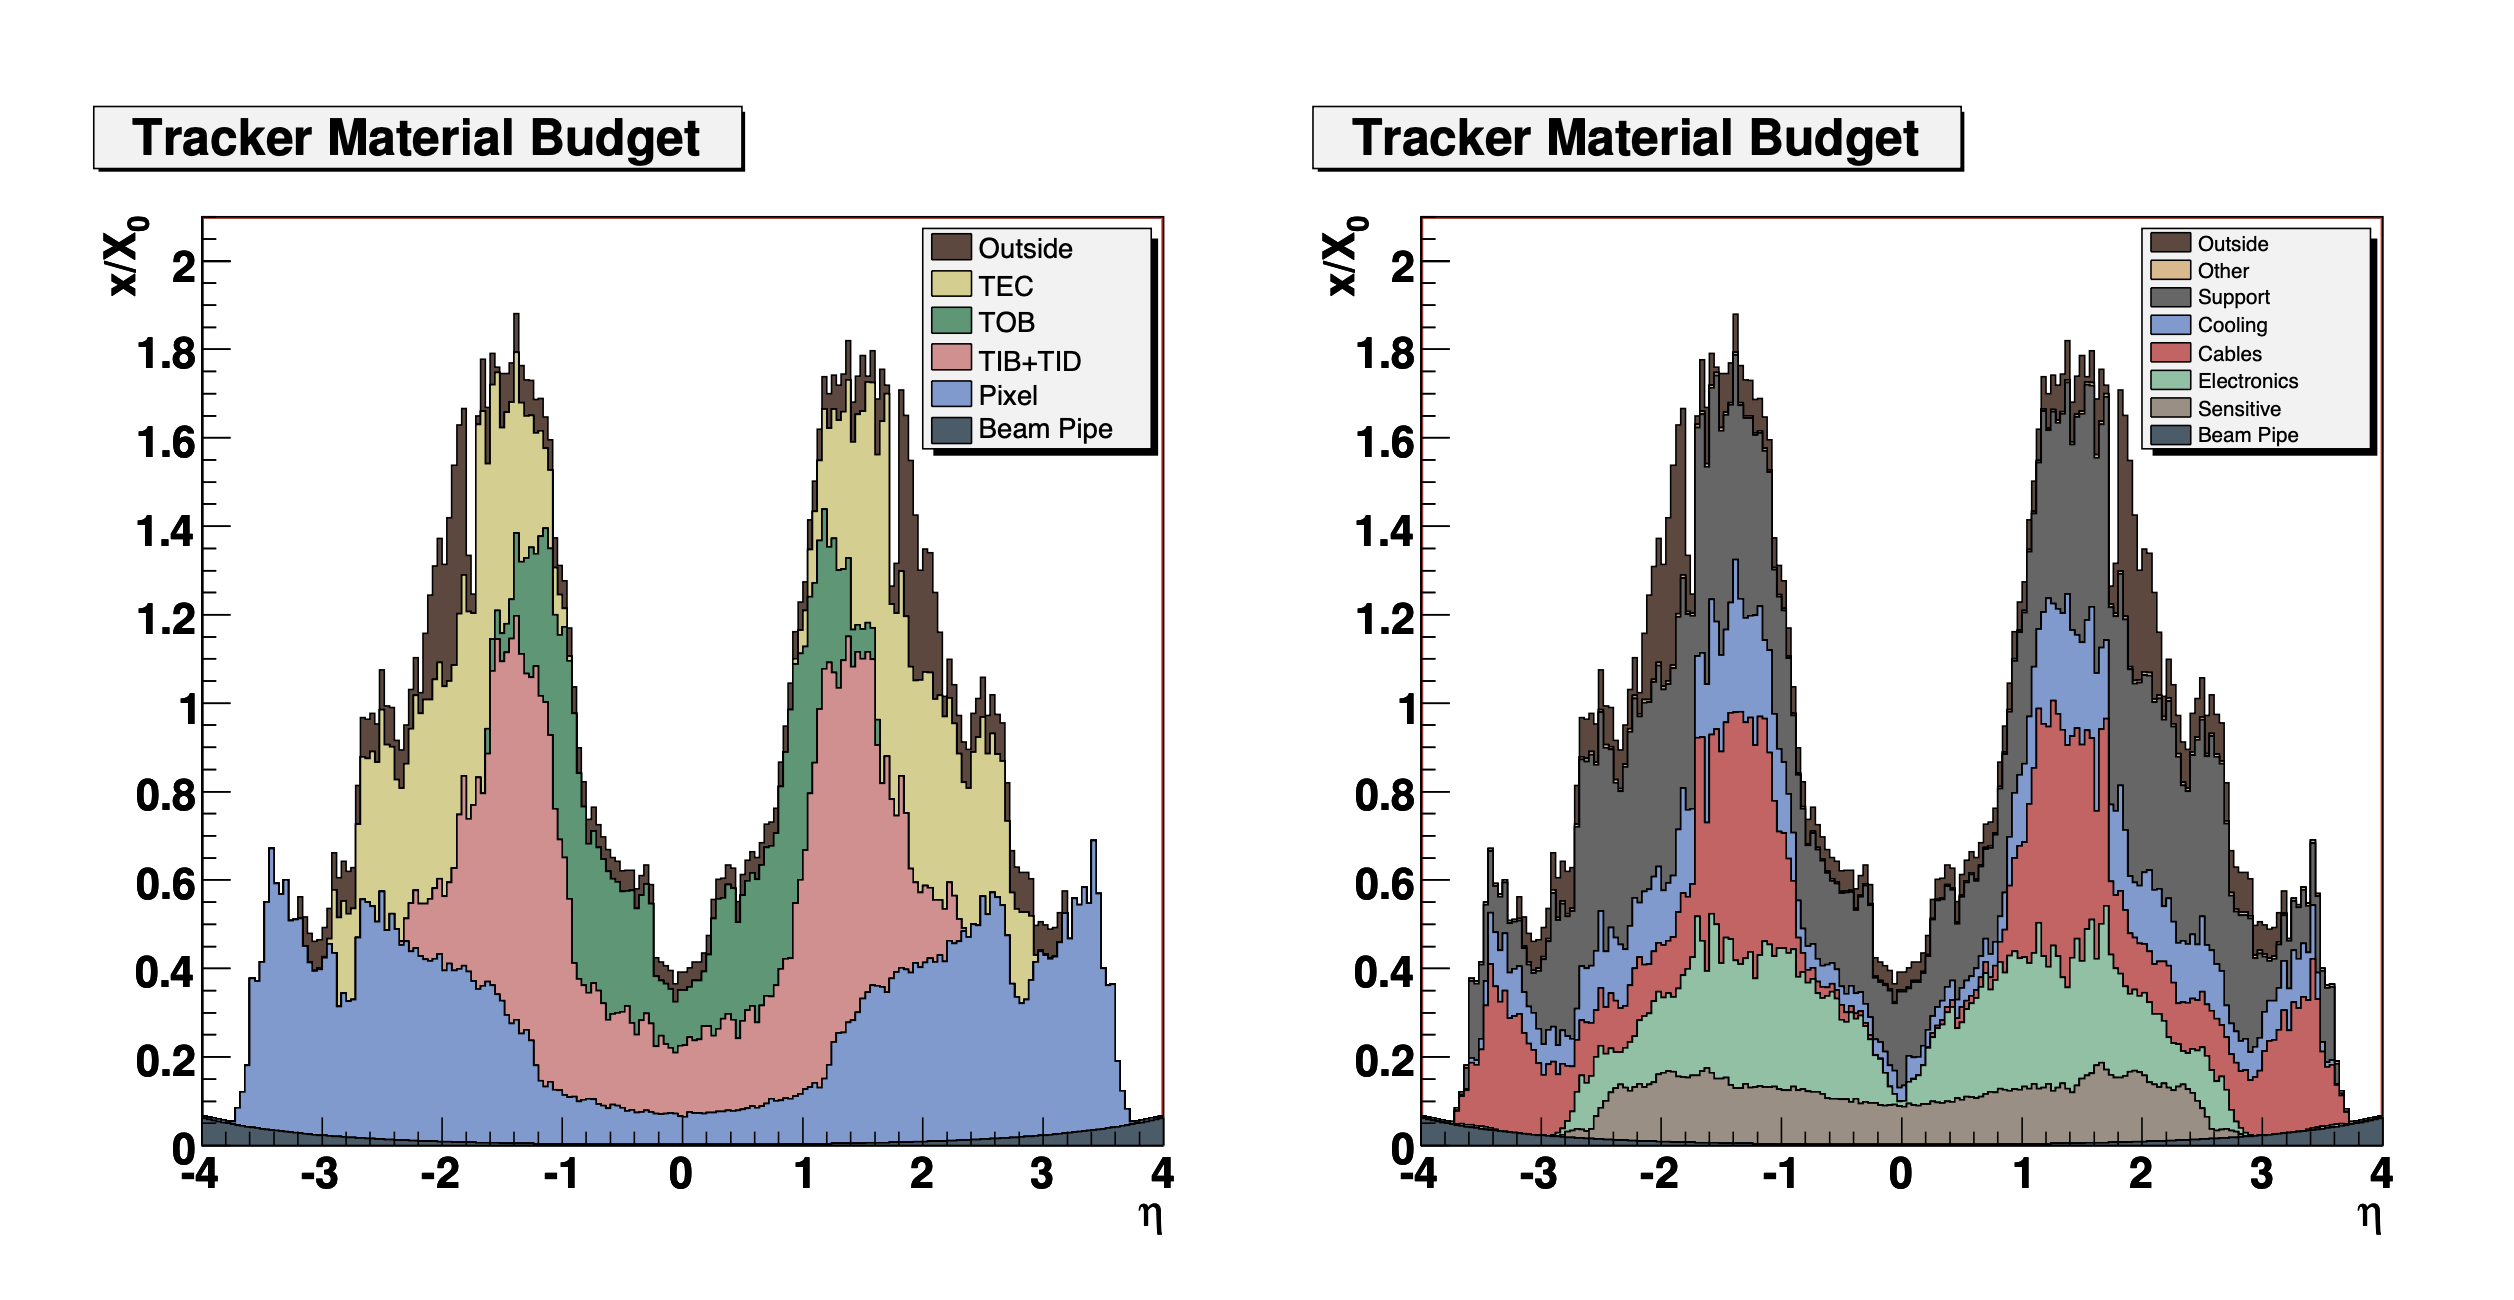
\includegraphics[width=0.98\textwidth]{chapters/2_experiment/figures/trackerMaterial.png}
    \caption{The material thickness of inner tracking system before ECAL.}
    \label{fig:exp:trackerMaterial}
\end{figure}


% pixel
The pixel detector, shown in the center of Figure~\ref{fig:exp:trigger}, is consist of three cylindrical layers of pixel detector modules at radii of 4.4, 7.3, and 10.2 cm, totaling 66 million pixels with area of 1 \si{\m \squared}. It is capable of producing three high precision 3D spacial hits for each charged particle. 

% tracker
 The silicon strip tracker system is right outside the pixel detector in the region of $20<r<116$ cm and $|z|<282$ cm. The tracker system has three parts: \acrfull{tibtid}, \acrfull{tob} and \acrfull{tec}, with a total of 9.3 million channels and 198 \si{\m \squared} active silicon area. The silicon strip modules in the barrel are lied out in cylindrical shapes with their strips parallel to the Z direction to measure $r-\phi$ coordinates. In comparison, those in the endcap region are in the shape of disks and place their strips in radial direction to measure the $Z-\phi$ coordinates. In addition to measuring the 2D coordinates, the first two cylinders of TIB and TOB, the first two disks of TID and TEC, as well as the fifth ring of TEC, are double-sided by placing a second micro-strip detector module back-to-back to the first module with a stereo angle of 100 mrad. This small stereo angle allows the measurement of the third spacial coordinates: $Z$ in the barrel (TIB and TOB) and $r$ on the endcap (TID and TEC). Such tracker design ensures to acquire at least 9 hits in the silicon strip tracker with at least 4 of them being stereo measurements. 

% Figure 3.3 shows the material budget of the CMS tracker in units of radiation length. It increases from 0.4 $\chi_0$ at $|\eta| =0$ to about 1.8 $\chi_0$ at $|\eta| =1.4$, beyond which it falls to about 1 $\chi_0$ at $|\eta| =2.5$.



\begin{figure}[ht]
    \centering
    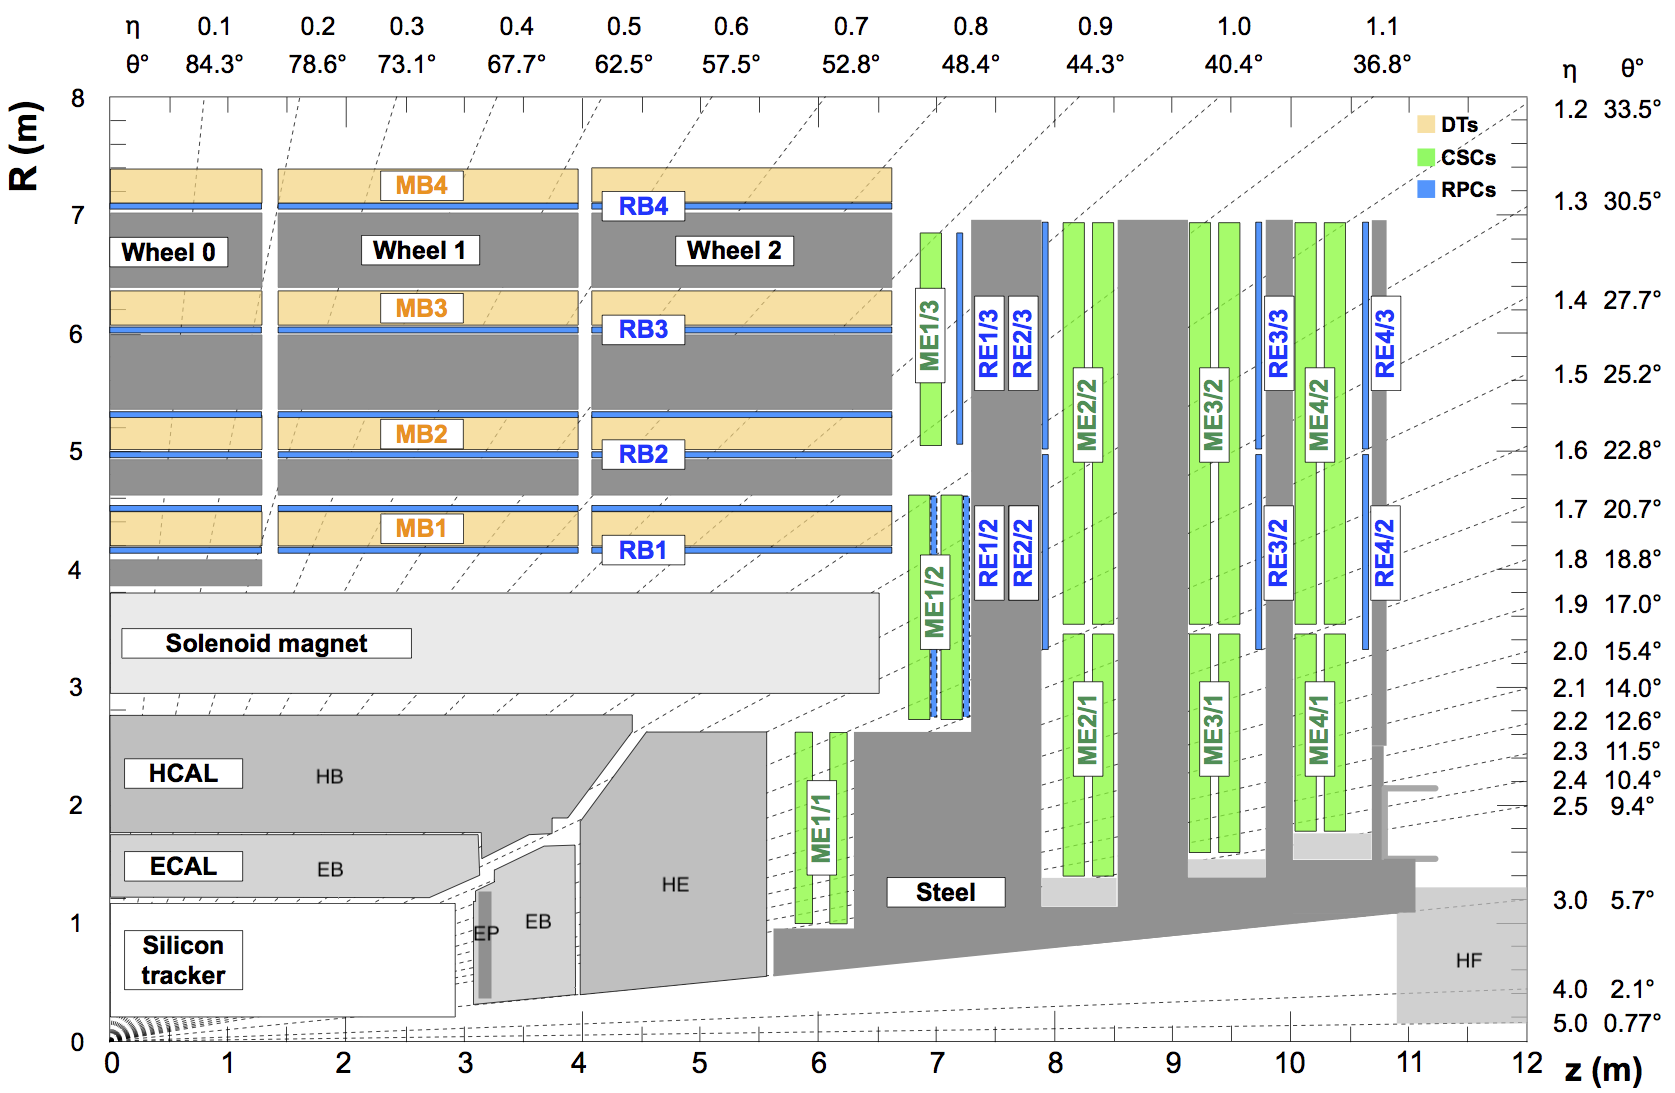
\includegraphics[width=0.98\textwidth]{chapters/2_experiment/figures/detectorLayout.png}
    \caption{The layout of the CMS tracker, ECAL, HCAL, Magnets and muon system on the Z-r plane \cite{cms:muonChamberWebsite}. The full coverage of pseudorapidity is up to $\eta=5$. The details of tracker is shown in Figure~\ref{fig:exp:tracker}. }
    \label{fig:exp:detectorLayout}
\end{figure}



\subsection{Electromagnetic Calorimeter (ECAL)}
%  overview
The CMS electromagnetic calorimeter (ECAL) \cite{cms:ecalTdr:CMS:1997ysd} is used to measure the energy of electromagnetic showers. As shown in Figure~\ref{fig:exp:detectorLayout}, ECAL is located right outside the tracking system discussed in the Section~\ref{sec:exp:trigger}. ECAL consists of the barrel part (EB), the endcap part (EE) and a preshower system (EP) in front of EE. EB and EE are hermetic homogeneous calorimeter made of lead tungstate crystals with \acrfull{apd} and \acrfull{vpt} as readout sensors respective, while the PS is a sampling calorimeter with lead-silicon alternating layers to enhance the spatial resolution in the EE region. The total ECAL material thickness is larger than 25 $\chi_0$ and about 1.1 $\lambda_I$.

% EB
The barrel part of the ECAL (EB) covers the pseudorapidity range of $|\eta|< 1.479$ and consists of 61200 crystals arranged in a 170x360 $\eta - \phi$ grid, with 8.14 $m^3$ of total crystal volume and 67.4 tons of weight. The crystals have a tapered shape mounted in a quasi-projective distribution, in which the crystal axis has 3\degree angle with respect to the vector from the origin to minimize chances of cracks aligned with the particle trajectories. The crystal cross-section corresponds to approximately $0.0174 \times 0.0174$ in $\eta - \phi$ or $22 \times 22$ $mm^2$ at the front face of crystal, and $26\times26$ $mm^2$ at the rear face. The crystal length is 230 mm corresponding to 25.8 $\chi_0$.

% EE
The endcaps (EE) cover the rapidity range $1.479 < |\eta| < 3.0$ and is consist of 7324 identically shaped crystals grouped in mechanical units of 5x5 crystals (supercrystals, or SCs), with 2.90 $m^3$ of total crystal volume and 24.0 tons of weight. The crystals are arranged in a rectangular x-y grid, with the crystals pointing at a focus 1300 mm beyond the interaction point, giving off-pointing angles ranging from 2 to 8 degrees. The crystals have a front face cross section $28.62\times28.62$ $mm^2$, a rear face cross section $30\times30$ $mm^2$ and a length of 220 mm corresponding to 24.7 $\chi_0$.

% preshower
A preshower detector (EP) is placed in front of EE in $1.479 < |\eta| < 2.6$ to increase the space resolution of electromagnetic showers and better identify neutral pions $\pi^0 \to \gamma \gamma$ in the endcap. EP is a sampling calorimeter with two lead-silicon layers. On each layer, the lead radiators initiate electromagnetic showers from incoming photons and electrons, while silicon strip sensors placed after each radiator measure the deposited energy and the transverse shower profiles. The directions of silicon strips on the two layers are orthogonal to each other. The material thickness of the first and second layer are 2 $\chi_0$ and 1 $\chi_0$ respective, with a total mechanical thickness of 20 cm.



\subsection{Hadron Calorimeter (HCAL)}
% overview
The CMS Hadron Calorimeter \cite{cms:hcalTdrCMS:1997xji} is used to measure the energy of hadrons and determine the missing transverse energy. HCAL consists of four parts: the HCAL in barrel region (HB) between ECAL and magnets, HCAL in the endcap region (HE), the forward hadronic calorimenter (HF) and a small section outside the magnetic (HO) in the barrel region to catch rare hadronic punch through before muon system. As shown in Figure~\ref{fig:exp:detectorLayout}, HB and HE are designed right outside the ECAL; FH is in the high pseudorapidity region outside the whole CMS endcap.

% HB, HE, HO
HB and HE are a sampling calorimeter covering $|\eta|< 1.3$, $1.3<|\eta|< 3.0$ respectively. They use brass absorber ($70\%$ Cu and $30\%$ Zn) and plastic scintillators for readout. HO covers the same $|\eta|< 1.3$ range as HB but uses iron as absorber enhance the material thickness in HB especially in the low $\eta$ region. With HO, the total material thickness of the HCAL is about 11.8 $\lambda_I$ make sure the hadronic leakage to muon is very rare. Totally, HCAL has about 7000 scintillators channels, granularity of which is $\Delta \eta \times \Delta \phi = 0.087 \times 0.087$ in the HB, OB and $1.3<|\eta|< 1.6$ part of HE and $\Delta \eta \times \Delta \phi = 0.017 \times 0.017$ in the rest part of HE.

% HF
HF is a sampling calorimeter covering $3.0 < |\eta| < 5$. It is essentially a cylindrical steel structure with an outer radius of 130.0 cm and with fibers piecing from the back in Z direction at two different depths. The front face of the calorimeter is located at 11.2 m from the interaction point. The absorber are made of steel installed perpendicular to beam pipe with a total material depth of 10 $\lambda_I$. The active material is quartz fibres (fused-silica core and polymer hard-cladding) installed in parallel with the beam pipe. When particle showers in the HF, a small part of Cherenkov light generated at the surface of quartz fibres is captured. To distinguish the electromagnetic shower vs hadronic shower, two different the penetration depth of fibers are used, long fiber span the entire HF, while short fibers start from 22 cm behind the HF front surface and extend to the back. These fibers are bundled to form $\Delta \phi \times \Delta \eta = 0.175 \times 0.175$ towers. 


\subsection{Muon System}
% overview
The CMS muon system \cite{cms:muonChamberTdr:CMS:1997iti} is designed outside the solenoid hosted in the return yoke to measure the tracks of muons. The system consists of barrel detector (MB) covering $|\eta|<1.2$ and endcap detectors (ME) covering $0.9 < |\eta| < 2.4$. 

% MB RPC
The barrel detector has 250 chambers in total which hosts 250 \acrfull{dt} and 480 \acrfull{rpc}. The chambers are  arranged in 4 concentric stations in the yoke, each of which is in turn divided into 5 wheels with 12 sectors on each wheel. The two inner most stations, labeled as MB1 and MB2 in Figure~\ref{fig:exp:detectorLayout}, has two RPCs sandwiching a DT, while The 2 outermost stations, MB3 and MB4 in Figure~\ref{fig:exp:detectorLayout}, consist of packages of a DT coupled to a layer on the inner side made of 1, 2, or 4 RPCs, depending on the sector and station.
Each DT in MB1, MB2 and MB3 has 12 layers of drift tubes divided into 3 groups of 4 consecutive layers or 3 superlayers. Two with wire parallel to Z direction measure $r-\phi$ coordinates, the middle one with wire perpendicular to Z direction measures $r-z$ coordinates. DTs in MB4 only have two superlayers for measurement of $r-\phi$ coordinates. RPCs are attached to DTs to improve the responding time necessary for triggers. Each RPC detector has a bakelite chamber with two 2 mm wide gaps and operates in avalanche mode biased by a high voltage. 

% ME
The endcap detector has 469 \acrfull{csc}s and 432 RPCs on two sides in the yokes that close the solenoid. The ME consists of 4 stations ME1-ME4. The disk of ME1 is divided into 3 concentric rings, while two rings for ME2-ME4. The details of the layout of CSCs and RPCs in ME are shown in Figure~\ref{fig:exp:detectorLayout}. Each CSC is trapezoidal in shape and consists of 6 gas gaps, each gap having a plane of radial cathode strips and a plane of anode wires running almost perpendicularly to the strips and measuring hits with 3D coordinates.





% ---------------------------------------
% section : Event Triggering
% ---------------------------------------
\section{Event Triggering}
\label{sec:exp:trigger}

% overview
CMS applies a two-tiered trigger system \cite{cms:trigger:Khachatryan:2016bia} to select event of interest. The \acrfull{l1t}, composed of custom hardware processors, uses information from the calorimeters and muon detectors to reduce the event rate from 40 MHz to 100 kHz, within a latency less than 4 $\mu s$. The second level, known as the \acrfull{hlt}, consists of a farm of processors running a version of the full event reconstruction software optimized for fast processing, and reduces the event rate from 100 kHz to 1 kHz and output for data storage.



\subsection{Level-1 Trigger}

\begin{figure}[ht]
    \centering
    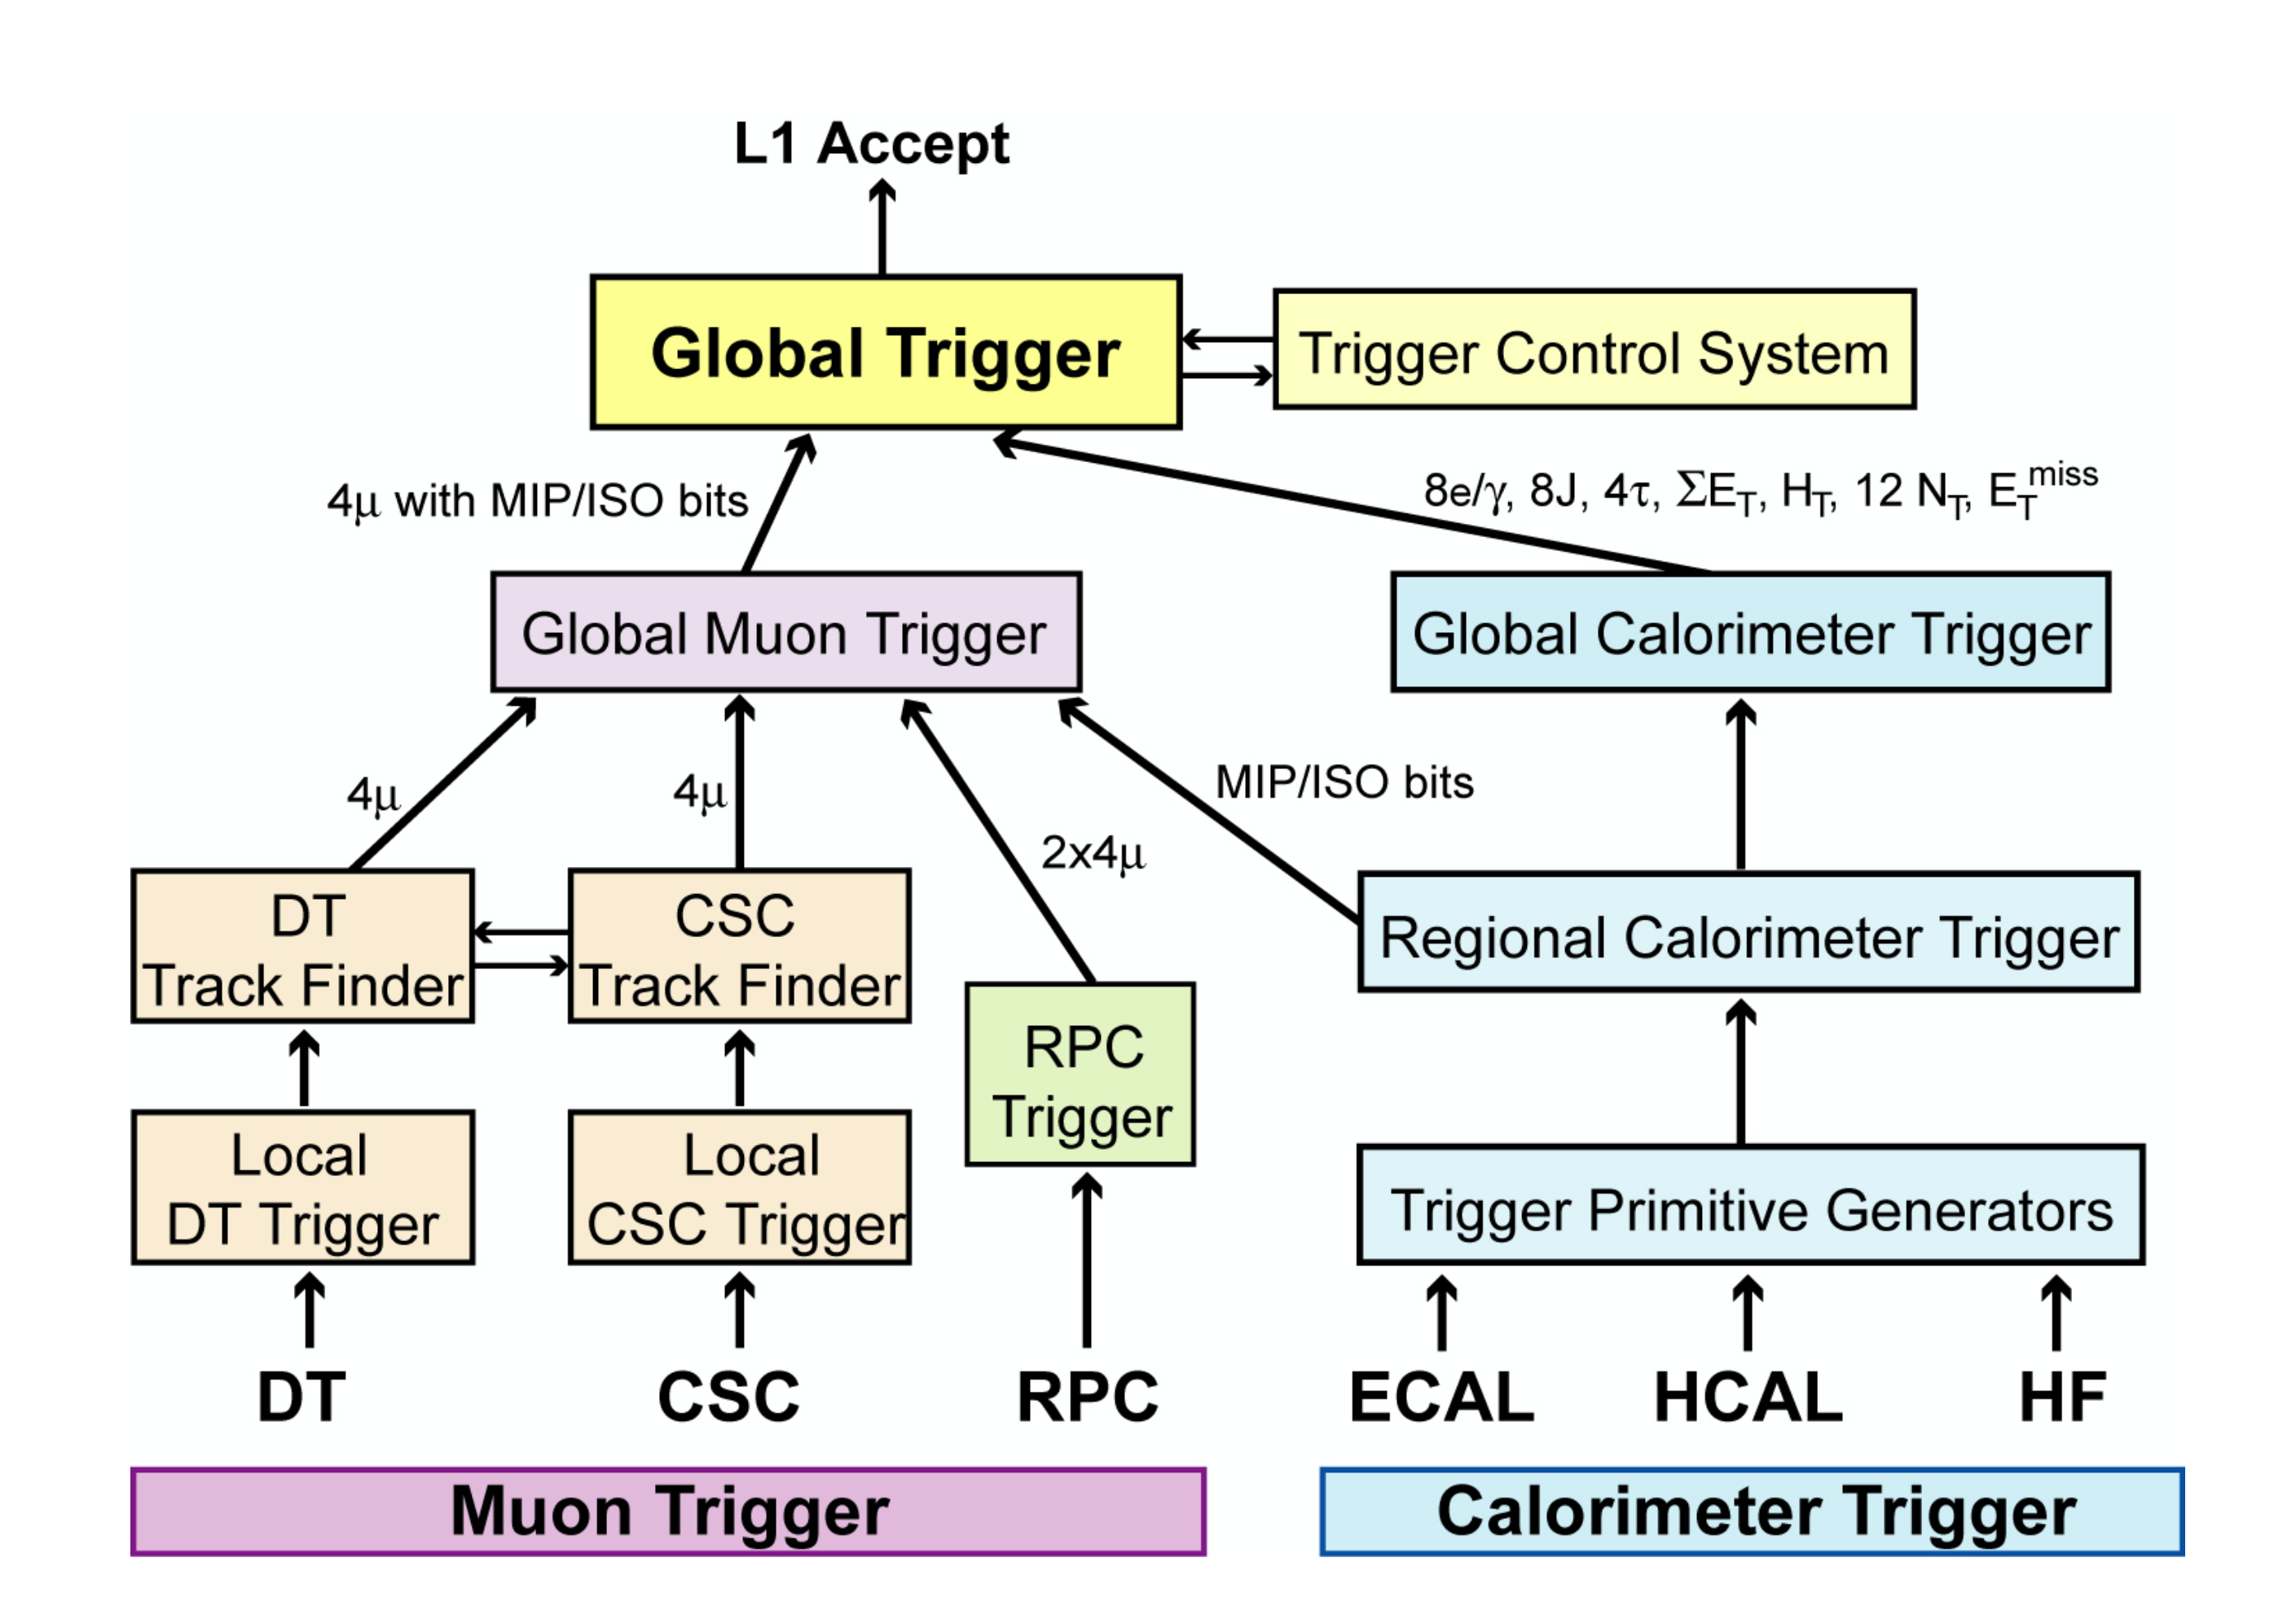
\includegraphics[width=0.8\textwidth]{chapters/2_experiment/figures/trigger.png}
    \caption{The logic structure of L1T.}
    %  Calorimeters and muon detectors raise local trigger primitives to compute a regional trigger signal. Then \acrfull{gmt} summarizes regional information from DT, SCS and PRC, while \acrfull{gct} concentrates the regional information from ECAL, HCAL and HF. Finally \acrfull{gt} makes the final decision based on the object orientated information from GMT and GCT and transport data in the sub-detectors to the HLT if L1T accept is made. 
    \label{fig:exp:trigger}
\end{figure}

% overview
L1 Trigger is designed to cope with the high collision frequency in the LHC, reducing the event rate from 40 MHz to 100 kHz, keeping only potential events of physics interest. To achieve this, L1 trigger is designed with three component: local, regional and global. The logic structure is shown in Figure~\ref{fig:exp:trigger}. The Local Triggers, also called \acrfull{tpg}, are based on energy deposits in calorimeter trigger towers and track segments or hit patterns in muon chambers. Regional Triggers combine their information and use pattern logic to determine ranked and sorted trigger objects such as electron or muon candidates in limited spatial regions. The \acrfull{gct} and \acrfull{gmt} determine the highest-rank calorimeter and muon objects across the entire experiment and transfer them to the \acrfull{gt}, the top entity of the Level-1 hierarchy. GT takes the decision to reject an event or to accept it for further evaluation by the HLT. The Level-1 Accept decision is communicated to the sub-detectors through the \acrfull{ttc} system. Before decisions arrive to the front-end, the raw data are stored in a FIFO pipelined memories in the front end electronics. Limited by the memory size, only a latency of \SI{3.2}{\us} is allowed between a given bunch crossing and the distribution of the L1T decision to the detector front-end electronics. The L1T electronics is housed partly on the detectors, partly in the underground control room located at a distance of approximately 90 m from the experimental cavern. 


% calo
The \acrfull{tpg} make up the first or local step of the Calorimeter Trigger pipeline. For triggering purposes, the calorimeters are subdivided in trigger towers. The TPGs sum the transverse energies measured in ECAL crystals or HCAL read-out towers to obtain the $E_T$ of the trigger tower and attach the correct bunch crossing number. The TPG electronics is integrated with the calorimeter read-out. The TPGs are transmitted through high-speed serial links to the Regional Calorimeter Trigger, which determines regional candidate electrons/photons, transverse energy sums, $\tau$-veto bits and information relevant for muons in the form of \acrfull{mip} and isolation bits. The Global Calorimeter Trigger determines the highest-rank calorimeter trigger objects across the entire calorimeter system, including 8 $e/\gamma$, 8 jet, 4 $\tau$, $\sum E_T$, $H_T$, 12 $n_j$, met.

% muon
All three muon systems – the DT, the CSC and the RPC – take part in the trigger. The barrel DT chambers provide local trigger information in the form of track segments in the $\phi$-projection and hit patterns in the $\eta$-projection. The endcap CSCs deliver 3-dimensional track segments. All chamber types also identify the bunch crossing from which an event originated. The Regional Muon Trigger consists of the DT and CSC Track Finders, which join segments to complete tracks and assign physical parameters to them. In addition, the RPC trigger chambers, which have excellent timing resolution, deliver their own track candidates based on regional hit patterns. The Global Muon Trigger then combines the information from the three sub-detectors and output 4 leading $\mu$ in the full coverage of muon system, achieving an improved momentum resolution and efficiency compared to the stand-alone systems.

% GT
The GT takes the decision to accept or reject an event at L1 based on trigger objects delivered by the GCT and GMT. The L1T accept decision is communicated to the sub-detectors through the TTC system. Then data corresponding to the triggered bunching crossing is readout from all front-end across the whole detector, as well as L1T objects from GT and send to the HLT.



\subsection{High Level Trigger}

The event selection at the HLT is performed in a similar way to that used in the offline processing. For each event, objects such as electrons, muons, and jets are reconstructed and identification criteria are applied in order to select only interested events.

% builder-filter
The HLT hardware consists of a single processor farm composed of commodity computers, the \acrfull{evf}, which runs Scientific Linux. The event filter farm consists of builder-filter units. In the builder units, individual event fragments from the detector are assembled to form complete events. Upon request from a filter unit, the builder unit ships an assembled event to the filter unit. The filter unit in turn unpacks the raw data into detector-specific data structures and performs the event reconstruction and trigger filtering. Associated builder and filter units are located in a single multi-core machine and communicate via shared memory. In total, the EVF executed on approximately 13,000 CPU cores at the end of 2012. On average, the HLT processing time per event is about 90 ms. EVF with 13,000 CPU cores allows a L1T output rate upto 100kHz. With a fixed L1T rate and increasing CPU cores, the allowed time budget for HLT can be expended. The output rate of HLT is limited by the event size and the computing and storage capacity of the offline system.

% filtering and storage
The filtering process uses the full precision of the data from the detector, and the selection is based on offline-quality reconstruction algorithms. It works by computing the a menu of HLT paths, in each of which a predefined process of object reconstruction and event selection is executed. If at least one of the HLT paths get past, the event will be accepted and sent to storage and offline processing. Upon HLT accept decision are made, the events are sent to the storage manager for archival storage. The event data are stored locally on disk and eventually transferred to the CMS Tier-0 computing center for offline processing and permanent storage. Events are grouped into a set of non-exclusive streams according to the HLT decisions.





% ---------------------------------------
% section : Object Reconstruction
% ---------------------------------------

\section{Object Reconstruction}
\label{sec:exp:reco}

The layer structure of CMS detector, tracking-ECAL-HCAL-Muon, is idea to particle flow reconstruction, which uses information from all subdetector systems and reconstruct each final state particles, including muon, egamma and hadrons. Based on the particle flow candidates, jets met are computed and BTag and hadronic tau are identified in the jet collections. 

Fig~\ref{fig:exp:pfa} illustrates the function of the sub dector and how different final state particles behave in them. Starting from the beam interaction region, particles first enter a tracker, in which charged-particle trajectories (tracks) and origins (vertices) are reconstructed from signals (hits) in the sensitive layers. The tracker is immersed in a magnetic field that bends the trajectories and allows the electric charges and momenta of charged particles to be measured. Electrons and photons are then absorbed in an electromagnetic calorimeter (ECAL). The corresponding electromagnetic showers are detected as clusters of energy recorded in neighbouring cells, from which the energy and direction of the particles can be determined. Charged and neutral hadrons may initiate a hadronic shower in the ECAL as well, which is subsequently fully absorbed in the hadron calorimeter (HCAL). The corresponding clusters are used to estimate their energies and directions. Muons and neutrinos traverse the calorimeters with little or no interactions. While neutrinos escape undetected, muons produce hits in additional tracking layers called muon detectors, located outside the calorimeters. As a result,  muons leaves tracks in the tracker and muon chamber with MIP in ECAL and HCAL. Electrons and phontons deposit energy in the ECAL with and without track correspondence respectively. Charged and neutral hadrons deposit energy in both ECAL and HCAL with and without track correspondence respectively. 

\begin{figure}[ht]
    \centering
    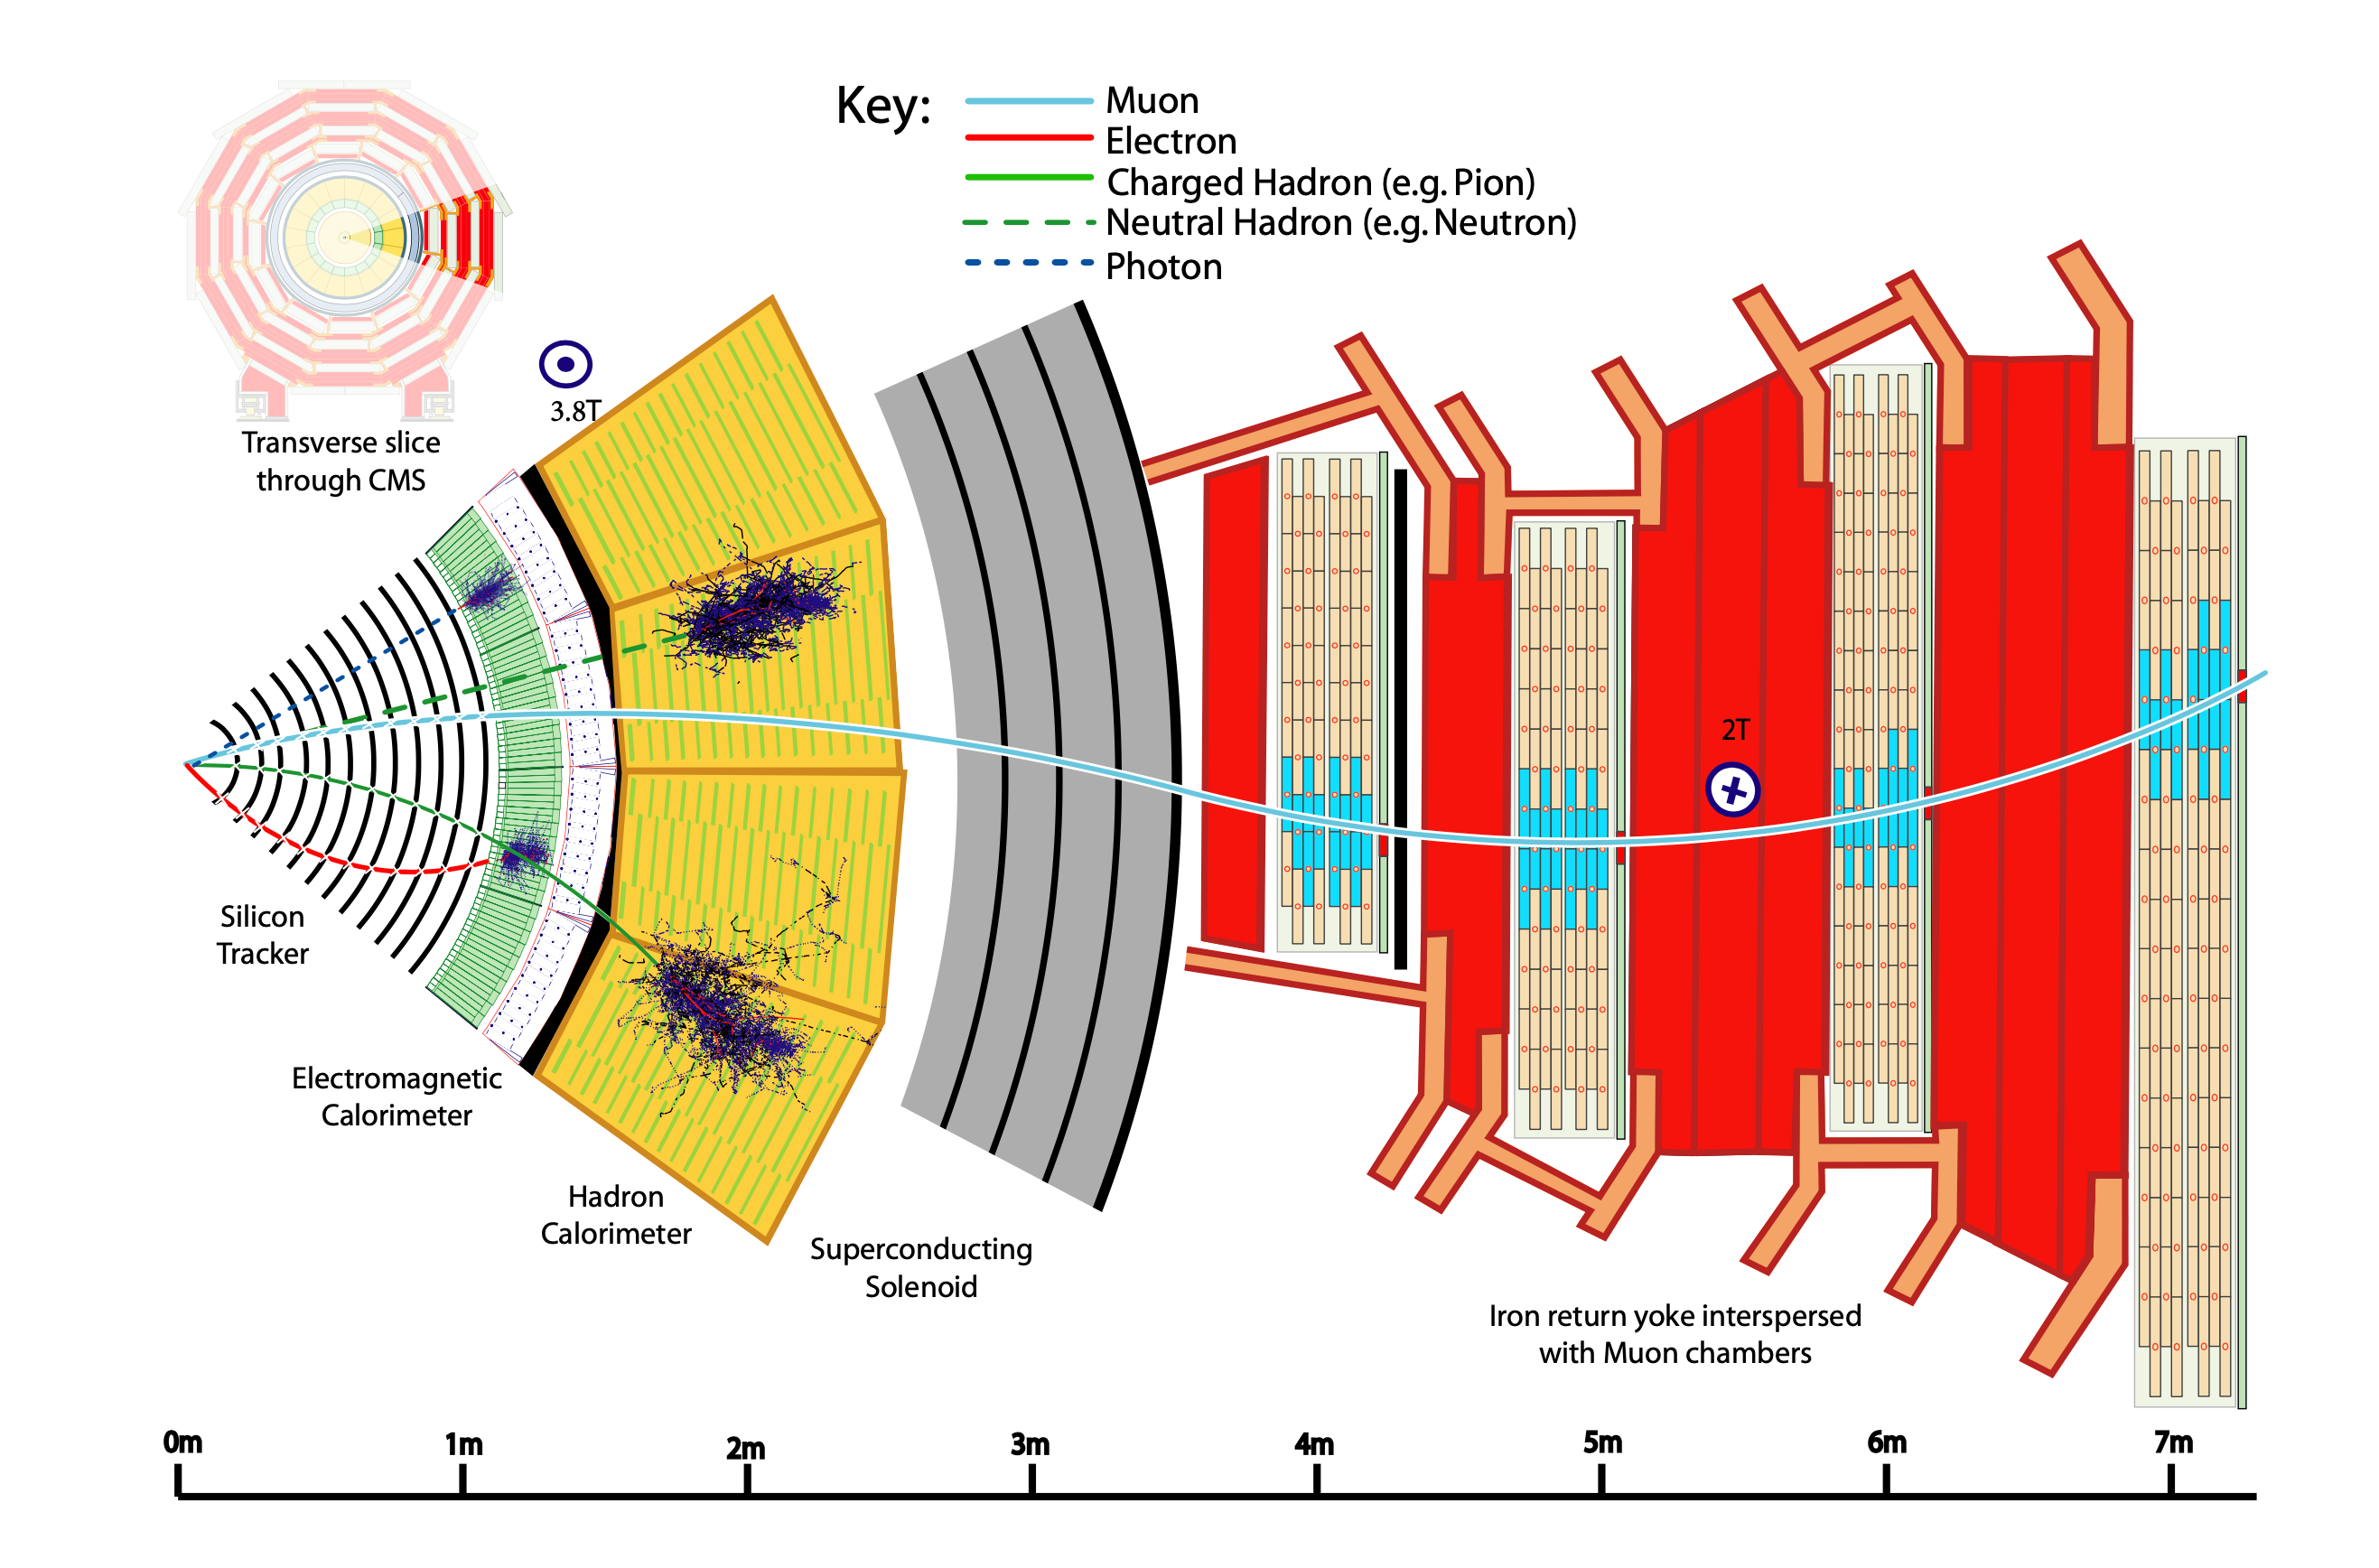
\includegraphics[width=0.8\textwidth]{chapters/2_experiment/figures/pfa.png}
    \caption{Caption}
    \label{fig:exp:pfa}
\end{figure}

The FPA begins with computing PF element in each subdetector: tracks in the tracker and muon chamber, clusters in ECAL and HCAL. Then PF elements in different subdetectors are linked to form PF Blocks via a linking process. PF Block summary the activity of potential particle candidate in each subdetector. The details of reconstruction of PF elements and their linking can be found in []. In the end, each PF blocks are identified into PF candidates, final state particles including muon, egamma and hadrons based on which JetMET, BTag and Tau ID are further computed.





\subsection{Muon}

The reconstruction of muon involves standalone reconstruction in the muon system, followed by globle muon reconstruction add trajectories in the tracker. The standalone reconstruction starts with the track segments in the individual muon chambers. The state vectors (track position, momentum, and direction) associated with the segments found in the innermost chambers are used to seed the muon trajectories, working from inside out, using the \acrfull{kf} technique \cite{tech:kf:Fruhwirth:1987fm}. The track parameters and the corresponding errors are updated at each step. The procedure is iterated until the outermost measurement surface of the muon system is reached. A backward Kalman-filter is then applied, working from outside in, and the track parameters are defined at the innermost muon station. Finally, the track is extrapolated to the nominal interaction point and a vertex-constrained fit to the track parameters is performed.

The global muon reconstruction consists in extending the muon trajectories to include hits in the silicon tracker. tarting from a standalone reconstructed muon, the muon trajectory is extrapolated from the innermost muon station to the outer tracker surface, taking into account the muon energy loss in the material and the effect of multiple scattering. This extrapolation and the associated uncertainty defines a region of interest in the tracker, where track candidates are seeded by hit doubles and reconstructed using Kalman-filter. A set of trajectory fits to the global hits are carried out to exact the muon momentum and impact parameters. This retain both prompt muons and muons from hadrons decays with the highest possible efficiency.

\begin{figure}[ht]
    \centering
    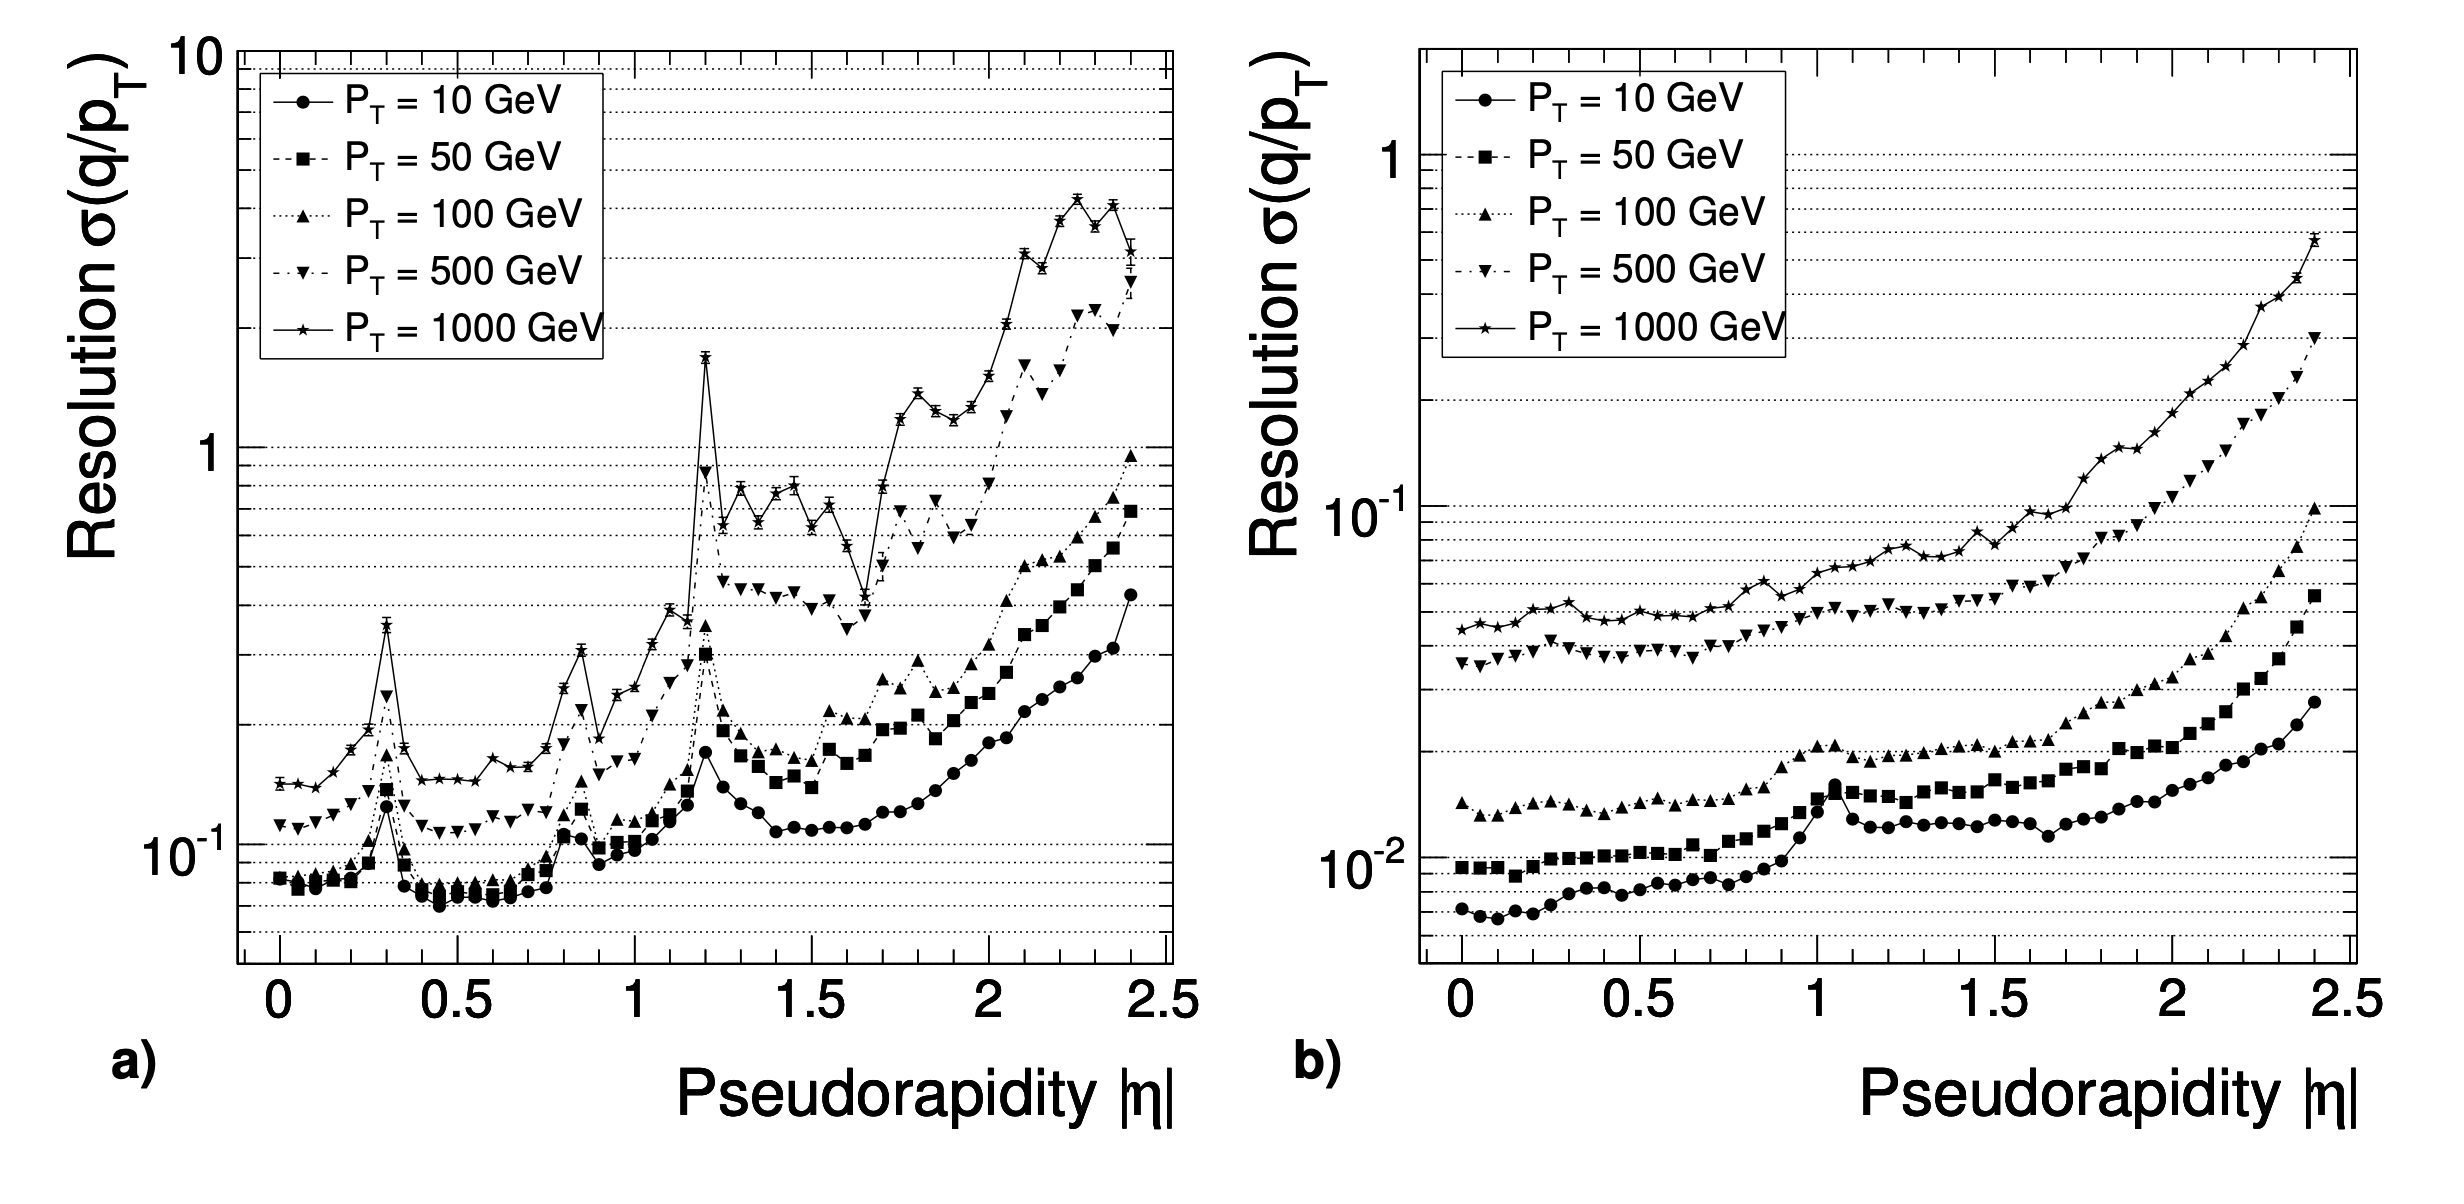
\includegraphics[width=0.95\textwidth]{chapters/2_experiment/figures/resMu.png}
    \caption{Momentum resolution as a function of }
    \label{fig:exp:resMu}
\end{figure}


Figure~\ref{fig:exp:resMu} shows the transverse momentum resolution of muons with different energies for standalone reconstruction algorithm (a) and the global reconstruction algorithm (b). A significant improvement is achieved when going from standalone to global muon reconstruction.





\subsection{EGamma}

\begin{figure}[ht]
    \centering
    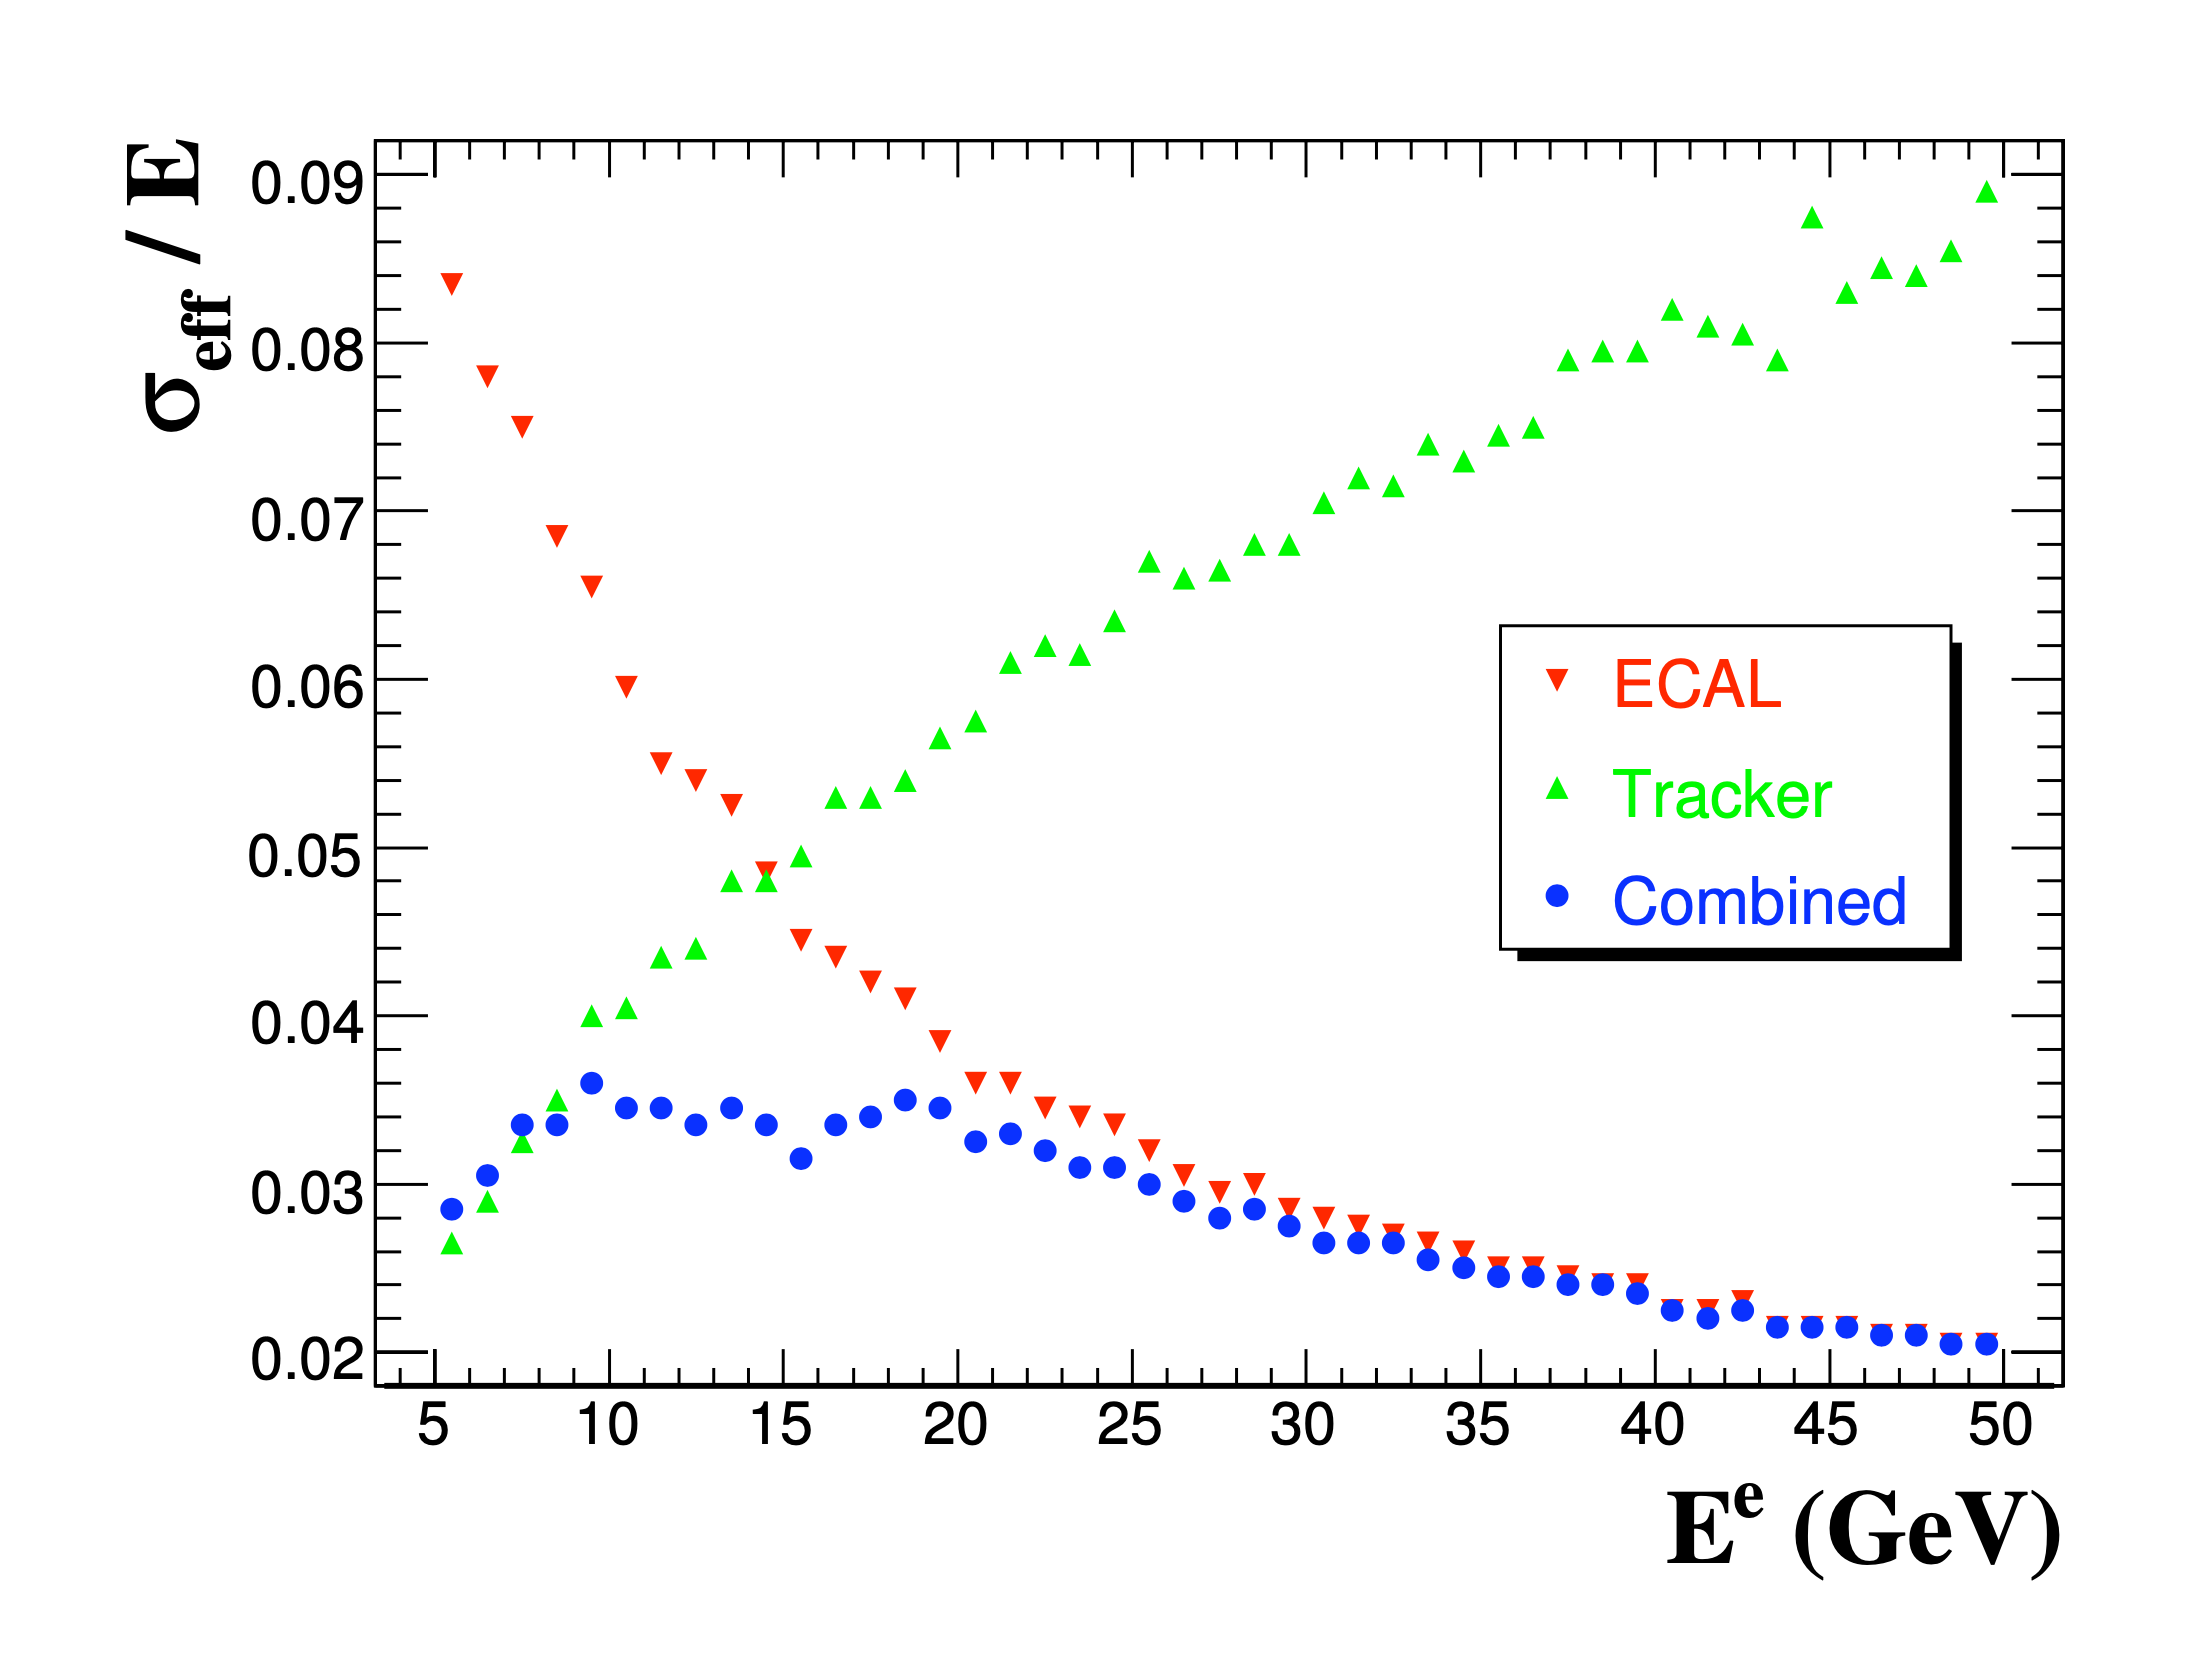
\includegraphics[width=0.5\textwidth]{chapters/2_experiment/figures/resEle.png}
    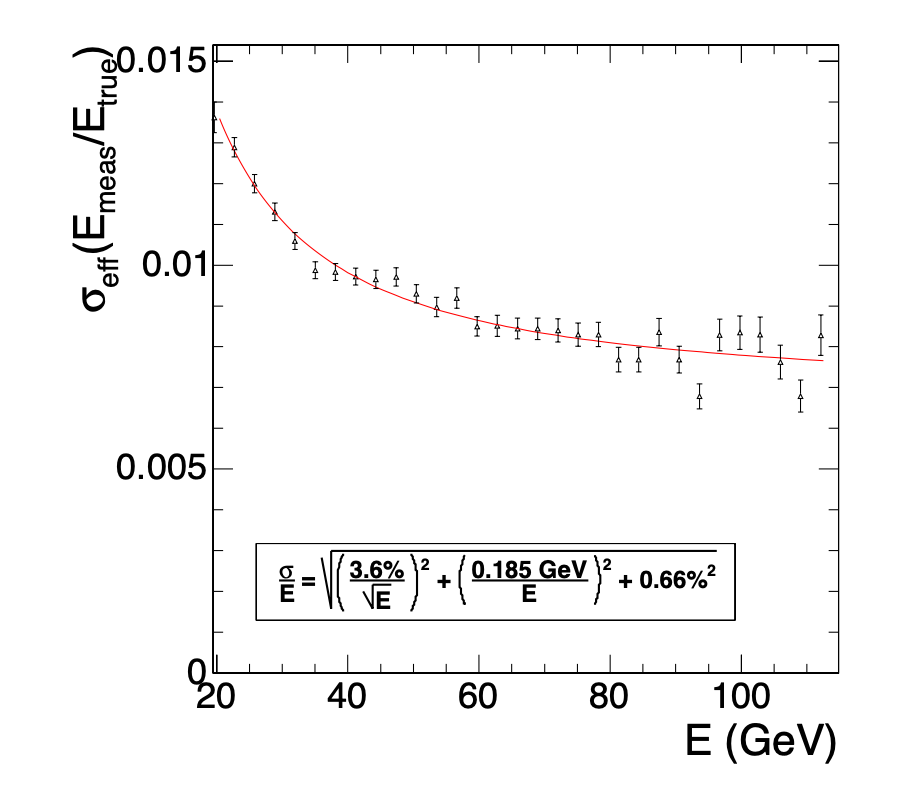
\includegraphics[width=0.42\textwidth]{chapters/2_experiment/figures/resGamma.png}
    \caption{Caption}
    \label{fig:exp:resEle}
\end{figure}

The electron reconstruction in CMS is hampered by the amount of tracker material which is discretely distributed in front of the ECAL. The material thickness varies strongly with $\eta$, raising from 0.3 $\chi_0$ at the central barrel to 1.5 $\chi_0$ at the barrel edge, then falling to 0.7 $\chi_0$ in the endcap inner edge. When electrons traversing the silicon layers of the pixel and inner tracker detectors, they radiate collections of bremsstrahlung photons and the energy reaches the ECAL spread in $\phi$. \cite{cms:tdr1:Bayatian:2006nff} provides an good illustration -- ''For electrons at $p^T=$10 GeV, about half of the electrons radiate away more than half of their energy before reaching the surface of the ECAL. In about 10$\%$ of the cases, more than 95$\%$ of the initial electron energy is radiated!'' Further more, the radiated photon can convert into electron-positron pairs, which are usually soft and trapped in the field loosing all energy in the end undetected.

The reconstruction of electron start with making superclusters of ECAL energy deposits. The superclustering algorithm is optimized for the scenarios of energy spread in $\phi$. The supercluster drives the finding of track seeds, which is hit doublets in pixel. If a seed compatible with the supercluster is found, tracks building begins inside-out with a nonlinear filter approach called \acrfull{gsf} \cite{tech:gsf:Adam:2005bya}. For supercluster linked with GFS tracks by particle-flow algorithm, an electron candidate is made and a fit to the GSF track and ECAL superclusters is used to extract the four-momentum measurement under the electron assumption. This not only provides combines the advantages of trackers in low energy region and the ECAL in the high energy region, but also connect the low energy and high energy region smoothly. The energy resolution of electrons using tracker, ECAL and combined is shown in Figure~\ref{fig:exp:resEle} left. For supercluster not linked to GFS tracks, an photon candidate is made and the energy is obtained from the sum of energy deposited in a supercluster of crystals. To quantify the lateral spread of photon shower, a variable R9 is defined as the ratio of sum energy in 3x3 crystals around the highest crystal and the total energy sum in the supercluster. Energy resolution of photons with R9 >0.943 is shown in Figure~\ref{fig:exp:resEle} right.



\subsection{hadrons}
Once muons, electrons, and isolated photons are identified and removed from the PF blocks, the remaining particles to be identified are hadrons from jet fragmentation and hadronization. These particles may be detected as charged hadrons and neutral hadrons, among which $\pi^0$ decays to two non-isolated photons. The ECAL and HCAL clusters not linked to any track give rise to non-isolated photons and neutral hadrons. Within the tracker acceptance ($|\eta|< 2.5$), all these ECAL clusters are turned into non-isolated photons and all these HCAL clusters are turned into neutral hadrons. 

Charge hadrons are made from the remaining calorimeter clusters and tracks. Each of the remaining HCAL clusters of the PF block is linked to one or several tracks and these tracks may in turn be linked to some of the remaining ECAL clusters. It is possible that calorimeter clusters also include unresolved FSR photons or close-by non-isolated neutral hadrons around charged hadrons. To identify unresolved neutral components around charged hadron, a match of calibrated calorimeter energy and tracker momentum is carried out. If the calibrated calorimetric energy is compatible with the sum of the track momenta, no neutral particle is identified. The charged-hadron momenta are redefined by further calibration taking into account information from both tracker and calorimeter. If the calibrated calorimetric energy is in excess of the sum of the track momenta by an amount larger than the expected calorimetric energy resolution for hadrons, the excess may be interpreted as the presence of photons and neutral hadrons. The excess energy is first treated as a non-isolated photon and subtracted from the ECAL energy. If ECAL energy alone is not enough to account for the excess, the remaining excess is treated as a neutral hadron. If the calibrated calorimeter energy is smaller than the tracking momentum, a search for non-isolated muon in the track projection is carried out with relaxed muon reconstruction standard and momentum of the reconstructed muons is subtracted before a re-compare.



\subsection{Jet and Met}

\begin{figure}[ht]
    \centering
    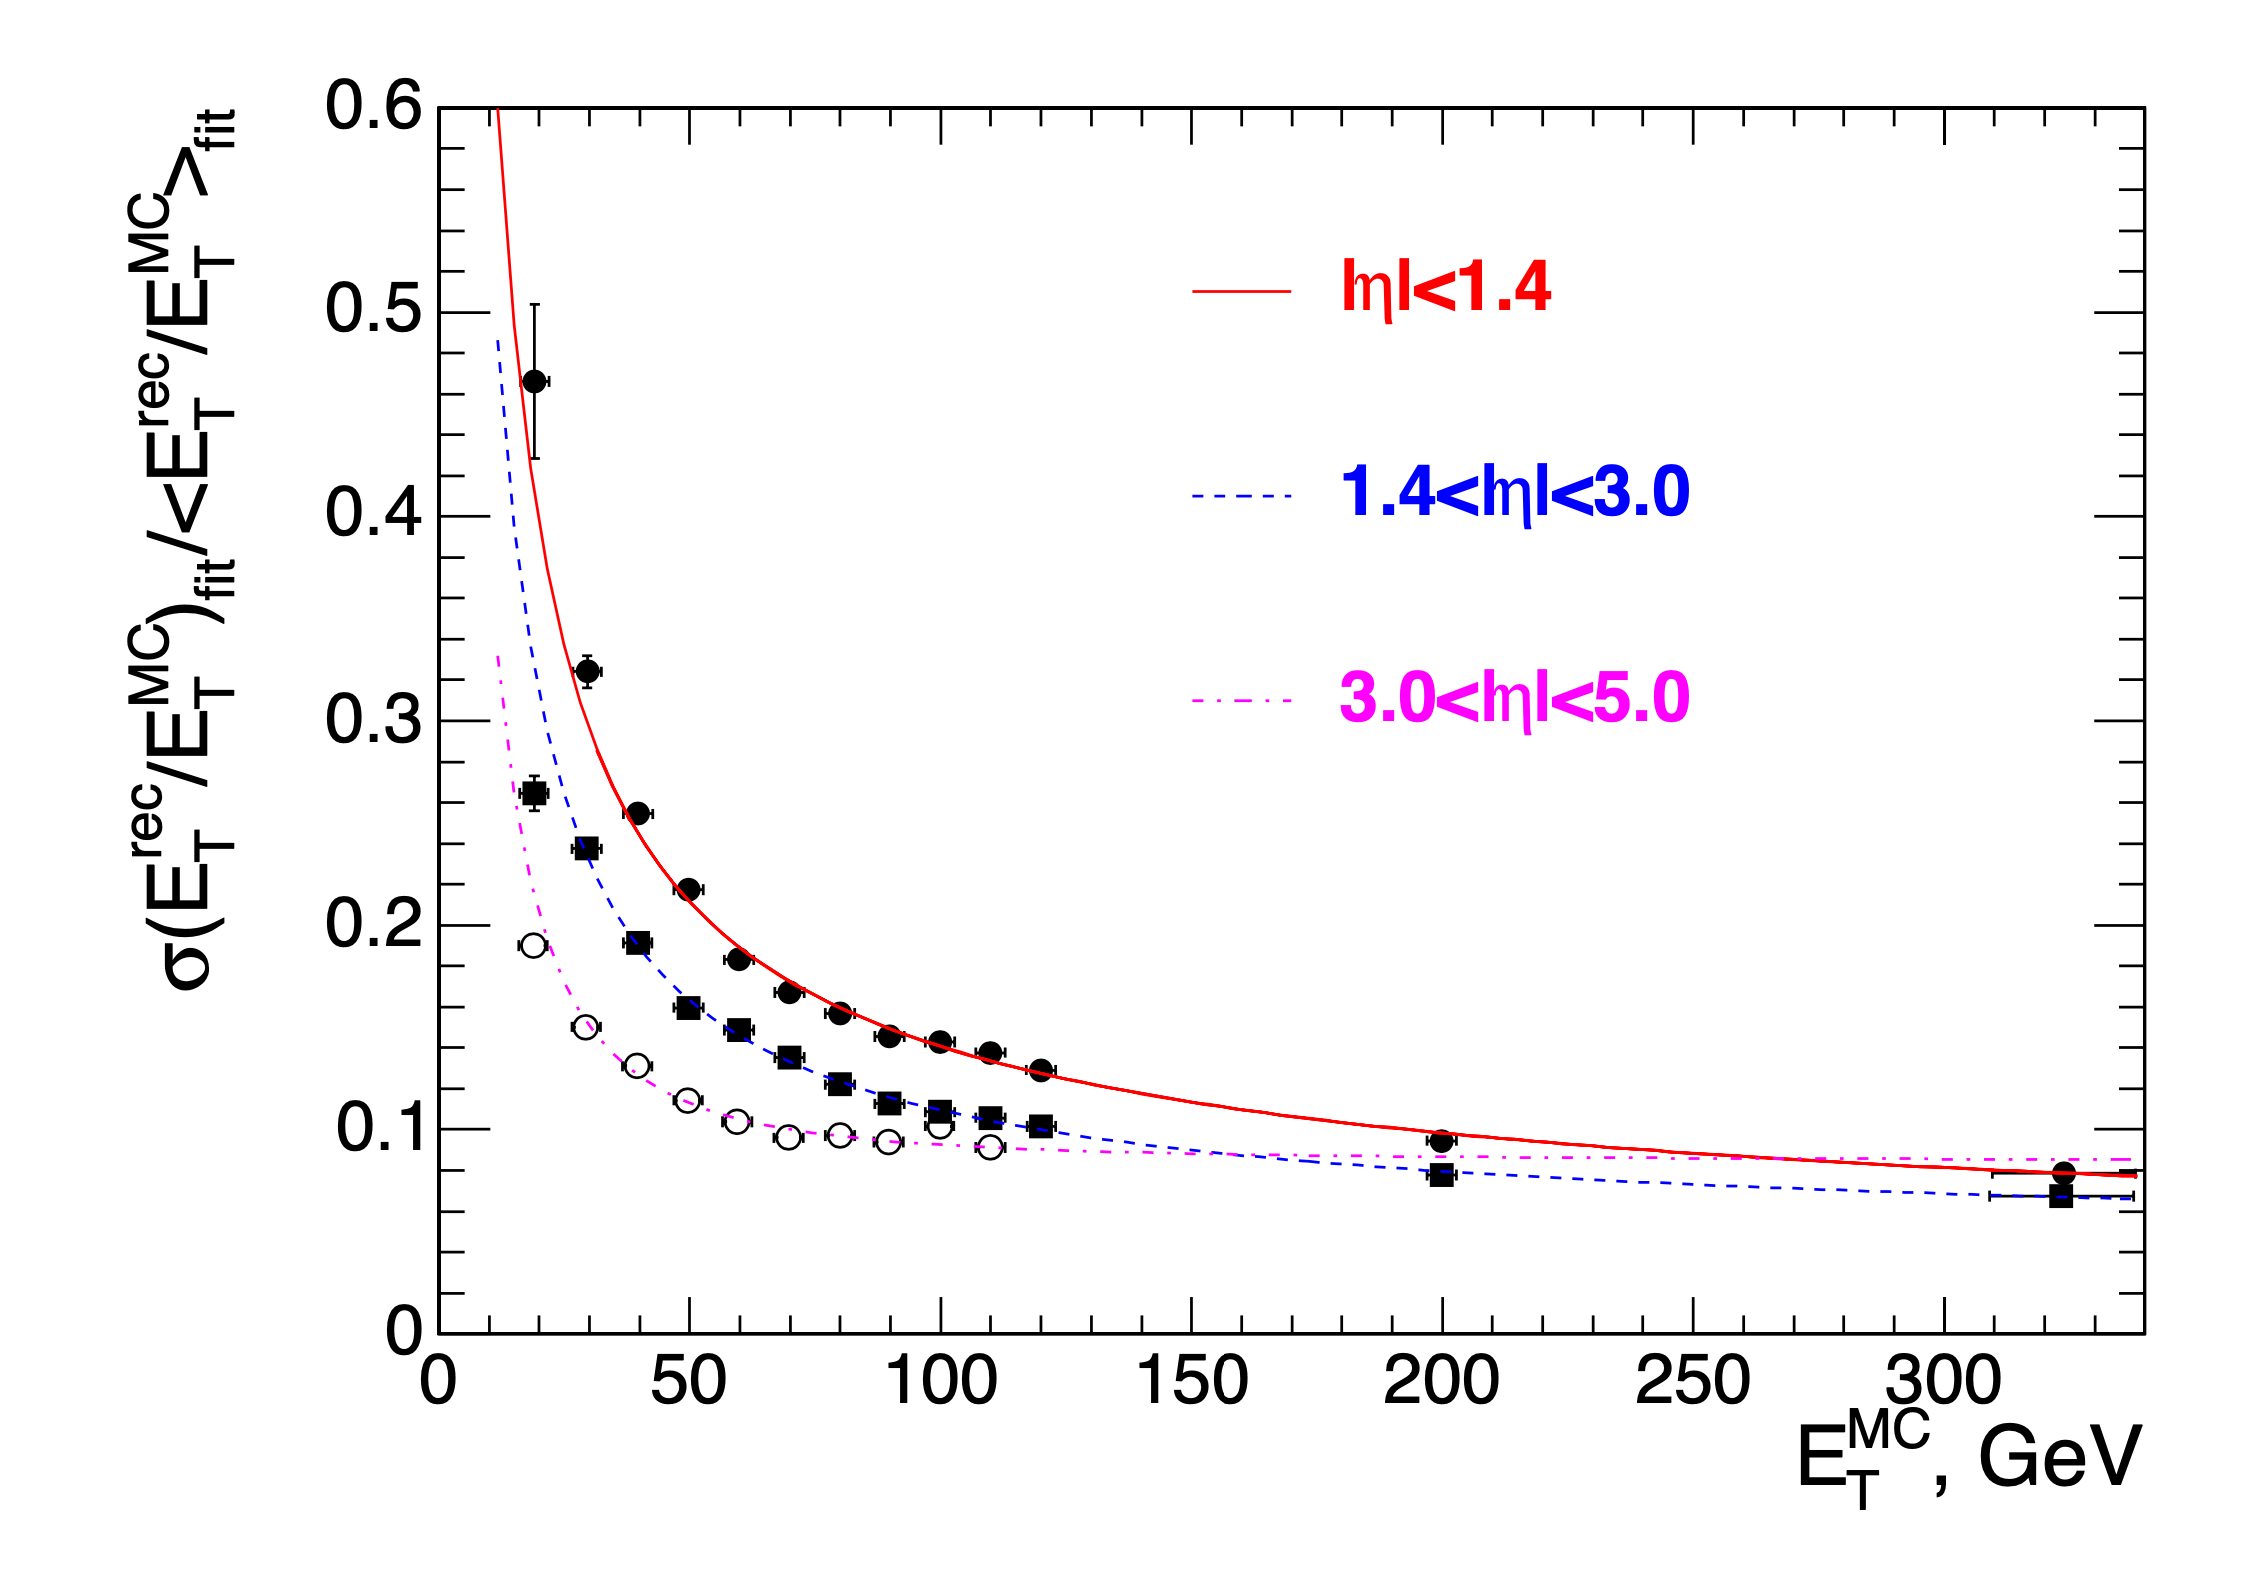
\includegraphics[width=0.6\textwidth]{chapters/2_experiment/figures/resJet.png}
    \caption{Caption}
    \label{fig:exp:resJet}
\end{figure}

Jet are reconstructed by clustering PF candidates using anti-kt algorithm \cite{tech:antikt:Cacciari:2008gp}. The energy resolution of jet is shown in Figure~\ref{fig:exp:resJet}. Met is computed by balancing the total visible transverse momentum. 



\subsection{bTagging}
Jets originated from heavy flavor quarks are tag via multi-variational method taking into account the displacement of secondary vertices.

\subsection{Tau ID}
 Jets originated from hadonic taus are tagged via iso-plus-striped algorithms.





